\documentclass[twoside]{book}

% Packages required by doxygen
\usepackage{calc}
\usepackage{doxygen}
\usepackage{graphicx}
\usepackage[utf8]{inputenc}
\usepackage{makeidx}
\usepackage{multicol}
\usepackage{multirow}
\usepackage{textcomp}
\usepackage[table]{xcolor}

% Font selection
\usepackage[T1]{fontenc}
\usepackage{mathptmx}
\usepackage[scaled=.90]{helvet}
\usepackage{courier}
\usepackage{amssymb}
\usepackage{sectsty}
\renewcommand{\familydefault}{\sfdefault}
\allsectionsfont{%
  \fontseries{bc}\selectfont%
  \color{darkgray}%
}
\renewcommand{\DoxyLabelFont}{%
  \fontseries{bc}\selectfont%
  \color{darkgray}%
}

% Page & text layout
\usepackage{geometry}
\geometry{%
  a4paper,%
  top=2.5cm,%
  bottom=2.5cm,%
  left=2.5cm,%
  right=2.5cm%
}
\tolerance=750
\hfuzz=15pt
\hbadness=750
\setlength{\emergencystretch}{15pt}
\setlength{\parindent}{0cm}
\setlength{\parskip}{0.2cm}
\makeatletter
\renewcommand{\paragraph}{%
  \@startsection{paragraph}{4}{0ex}{-1.0ex}{1.0ex}{%
    \normalfont\normalsize\bfseries\SS@parafont%
  }%
}
\renewcommand{\subparagraph}{%
  \@startsection{subparagraph}{5}{0ex}{-1.0ex}{1.0ex}{%
    \normalfont\normalsize\bfseries\SS@subparafont%
  }%
}
\makeatother

% Headers & footers
\usepackage{fancyhdr}
\pagestyle{fancyplain}
\fancyhead[LE]{\fancyplain{}{\bfseries\thepage}}
\fancyhead[CE]{\fancyplain{}{}}
\fancyhead[RE]{\fancyplain{}{\bfseries\leftmark}}
\fancyhead[LO]{\fancyplain{}{\bfseries\rightmark}}
\fancyhead[CO]{\fancyplain{}{}}
\fancyhead[RO]{\fancyplain{}{\bfseries\thepage}}
\fancyfoot[LE]{\fancyplain{}{}}
\fancyfoot[CE]{\fancyplain{}{}}
\fancyfoot[RE]{\fancyplain{}{\bfseries\scriptsize Generated on Sun Sep 15 2013 09\-:55\-:48 for My Project by Doxygen }}
\fancyfoot[LO]{\fancyplain{}{\bfseries\scriptsize Generated on Sun Sep 15 2013 09\-:55\-:48 for My Project by Doxygen }}
\fancyfoot[CO]{\fancyplain{}{}}
\fancyfoot[RO]{\fancyplain{}{}}
\renewcommand{\footrulewidth}{0.4pt}
\renewcommand{\chaptermark}[1]{%
  \markboth{#1}{}%
}
\renewcommand{\sectionmark}[1]{%
  \markright{\thesection\ #1}%
}

% Indices & bibliography
\usepackage{natbib}
\usepackage[titles]{tocloft}
\setcounter{tocdepth}{3}
\setcounter{secnumdepth}{5}
\makeindex

% Hyperlinks (required, but should be loaded last)
\usepackage{ifpdf}
\ifpdf
  \usepackage[pdftex,pagebackref=true]{hyperref}
\else
  \usepackage[ps2pdf,pagebackref=true]{hyperref}
\fi
\hypersetup{%
  colorlinks=true,%
  linkcolor=blue,%
  citecolor=blue,%
  unicode%
}

% Custom commands
\newcommand{\clearemptydoublepage}{%
  \newpage{\pagestyle{empty}\cleardoublepage}%
}


%===== C O N T E N T S =====

\begin{document}

% Titlepage & ToC
\hypersetup{pageanchor=false}
\pagenumbering{roman}
\begin{titlepage}
\vspace*{7cm}
\begin{center}%
{\Large My Project }\\
\vspace*{1cm}
{\large Generated by Doxygen 1.8.5}\\
\vspace*{0.5cm}
{\small Sun Sep 15 2013 09:55:48}\\
\end{center}
\end{titlepage}
\clearemptydoublepage
\tableofcontents
\clearemptydoublepage
\pagenumbering{arabic}
\hypersetup{pageanchor=true}

%--- Begin generated contents ---
\chapter{Namespace Index}
\section{Packages}
Here are the packages with brief descriptions (if available)\-:\begin{DoxyCompactList}
\item\contentsline{section}{\hyperlink{namespace_engine}{Engine} }{\pageref{namespace_engine}}{}
\item\contentsline{section}{\hyperlink{namespace_engine_1_1_properties}{Engine.\-Properties} }{\pageref{namespace_engine_1_1_properties}}{}
\end{DoxyCompactList}

\chapter{Hierarchical Index}
\section{Class Hierarchy}
This inheritance list is sorted roughly, but not completely, alphabetically\-:\begin{DoxyCompactList}
\item \contentsline{section}{Engine.\-App}{\pageref{class_engine_1_1_app}}{}
\item Form\begin{DoxyCompactList}
\item \contentsline{section}{Engine.\-Form1}{\pageref{class_engine_1_1_form1}}{}
\end{DoxyCompactList}
\item \contentsline{section}{Engine.\-Loop}{\pageref{class_engine_1_1_loop}}{}
\item \contentsline{section}{Engine.\-Matrix}{\pageref{class_engine_1_1_matrix}}{}
\item \contentsline{section}{Engine.\-Message}{\pageref{struct_engine_1_1_message}}{}
\item \contentsline{section}{Engine.\-Screen}{\pageref{class_engine_1_1_screen}}{}
\item \contentsline{section}{Engine.\-Time}{\pageref{class_engine_1_1_time}}{}
\item \contentsline{section}{Engine.\-Vector2}{\pageref{struct_engine_1_1_vector2}}{}
\item \contentsline{section}{Engine.\-Vector3}{\pageref{struct_engine_1_1_vector3}}{}
\item \contentsline{section}{Engine.\-Vector4}{\pageref{struct_engine_1_1_vector4}}{}
\end{DoxyCompactList}

\chapter{Class Index}
\section{Class List}
Here are the classes, structs, unions and interfaces with brief descriptions\-:\begin{DoxyCompactList}
\item\contentsline{section}{\hyperlink{class_engine_1_1_app}{Engine.\-App} }{\pageref{class_engine_1_1_app}}{}
\item\contentsline{section}{\hyperlink{class_engine_1_1_form1}{Engine.\-Form1} }{\pageref{class_engine_1_1_form1}}{}
\item\contentsline{section}{\hyperlink{class_engine_1_1_loop}{Engine.\-Loop} }{\pageref{class_engine_1_1_loop}}{}
\item\contentsline{section}{\hyperlink{class_engine_1_1_matrix}{Engine.\-Matrix} }{\pageref{class_engine_1_1_matrix}}{}
\item\contentsline{section}{\hyperlink{struct_engine_1_1_message}{Engine.\-Message} }{\pageref{struct_engine_1_1_message}}{}
\item\contentsline{section}{\hyperlink{class_engine_1_1_screen}{Engine.\-Screen} }{\pageref{class_engine_1_1_screen}}{}
\item\contentsline{section}{\hyperlink{class_engine_1_1_time}{Engine.\-Time} }{\pageref{class_engine_1_1_time}}{}
\item\contentsline{section}{\hyperlink{struct_engine_1_1_vector2}{Engine.\-Vector2} }{\pageref{struct_engine_1_1_vector2}}{}
\item\contentsline{section}{\hyperlink{struct_engine_1_1_vector3}{Engine.\-Vector3} }{\pageref{struct_engine_1_1_vector3}}{}
\item\contentsline{section}{\hyperlink{struct_engine_1_1_vector4}{Engine.\-Vector4} }{\pageref{struct_engine_1_1_vector4}}{}
\end{DoxyCompactList}

\chapter{Namespace Documentation}
\hypertarget{namespace_engine}{\section{Package Engine}
\label{namespace_engine}\index{Engine@{Engine}}
}
\subsection*{Namespaces}
\begin{DoxyCompactItemize}
\item 
package \hyperlink{namespace_engine_1_1_properties}{Properties}
\end{DoxyCompactItemize}
\subsection*{Classes}
\begin{DoxyCompactItemize}
\item 
class \hyperlink{class_engine_1_1_app}{App}
\item 
class \hyperlink{class_engine_1_1_screen}{Screen}
\item 
class \hyperlink{class_engine_1_1_form1}{Form1}
\item 
struct \hyperlink{struct_engine_1_1_message}{Message}
\item 
class \hyperlink{class_engine_1_1_loop}{Loop}
\item 
class {\bfseries Mathf}
\item 
class \hyperlink{class_engine_1_1_matrix}{Matrix}
\item 
struct \hyperlink{struct_engine_1_1_vector3}{Vector3}
\item 
struct \hyperlink{struct_engine_1_1_vector2}{Vector2}
\item 
struct \hyperlink{struct_engine_1_1_vector4}{Vector4}
\item 
class {\bfseries Program}
\item 
class \hyperlink{class_engine_1_1_time}{Time}
\end{DoxyCompactItemize}
\subsection*{Enumerations}
\begin{DoxyCompactItemize}
\item 
enum {\bfseries Projection} \{ \\*
{\bfseries Center}, 
{\bfseries Upper\-Left}, 
{\bfseries Upper\-Right}, 
{\bfseries Lower\-Left}, 
\\*
{\bfseries Lower\-Right}
 \}
\end{DoxyCompactItemize}

\hypertarget{namespace_engine_1_1_properties}{\section{Package Engine.\-Properties}
\label{namespace_engine_1_1_properties}\index{Engine.\-Properties@{Engine.\-Properties}}
}
\subsection*{Classes}
\begin{DoxyCompactItemize}
\item 
class {\bfseries Resources}
\begin{DoxyCompactList}\small\item\em A strongly-\/typed resource class, for looking up localized strings, etc. \end{DoxyCompactList}\item 
class {\bfseries Settings}
\end{DoxyCompactItemize}

\chapter{Class Documentation}
\hypertarget{class_engine_1_1_app}{\section{Engine.\-App Class Reference}
\label{class_engine_1_1_app}\index{Engine.\-App@{Engine.\-App}}
}
\subsection*{Static Public Member Functions}
\begin{DoxyCompactItemize}
\item 
\hypertarget{class_engine_1_1_app_a315fe14a9f658db6b6fa19d2f9debbd1}{static Open\-G\-L\-Control {\bfseries Init} ()}\label{class_engine_1_1_app_a315fe14a9f658db6b6fa19d2f9debbd1}

\item 
\hypertarget{class_engine_1_1_app_a3135cd61cb9c794e29d14feecc6e2047}{static void {\bfseries Set\-Projection2\-D} (float width, float height, Projection projection=Projection.\-Center)}\label{class_engine_1_1_app_a3135cd61cb9c794e29d14feecc6e2047}

\item 
\hypertarget{class_engine_1_1_app_ad80d42c948b067df7e8ddc8f5334be1f}{static void {\bfseries Set\-Projection2\-D} (float left, float right, float bottom, float top)}\label{class_engine_1_1_app_ad80d42c948b067df7e8ddc8f5334be1f}

\end{DoxyCompactItemize}


The documentation for this class was generated from the following file\-:\begin{DoxyCompactItemize}
\item 
C\-:/\-Users/\-Lucas/\-Documents/\-Git\-Hub/\-Engine/\-Engine/App.\-cs\end{DoxyCompactItemize}

\hypertarget{class_engine_1_1_form1}{\section{Engine.\-Form1 Class Reference}
\label{class_engine_1_1_form1}\index{Engine.\-Form1@{Engine.\-Form1}}
}
Inheritance diagram for Engine.\-Form1\-:\begin{figure}[H]
\begin{center}
\leavevmode
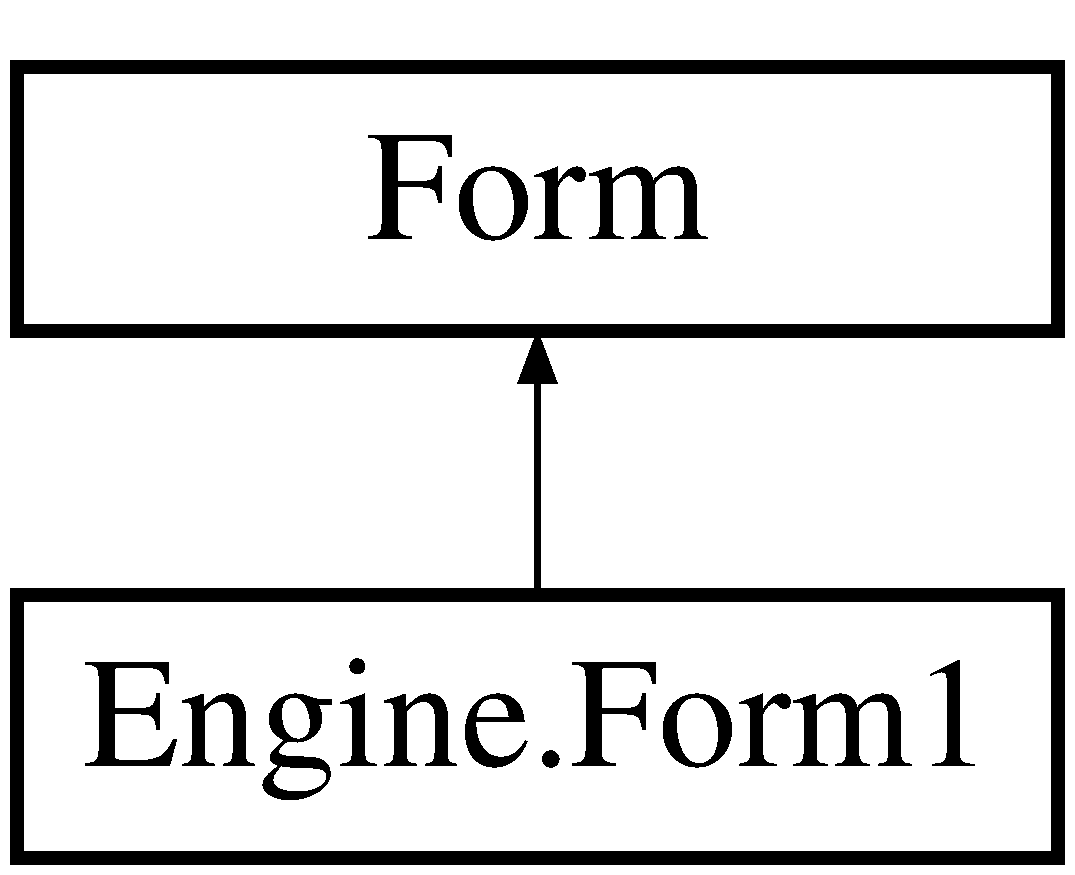
\includegraphics[height=2.000000cm]{class_engine_1_1_form1}
\end{center}
\end{figure}
\subsection*{Protected Member Functions}
\begin{DoxyCompactItemize}
\item 
\hypertarget{class_engine_1_1_form1_afab59b8eb76abcef16d87c52aaa5f783}{override void {\bfseries On\-Client\-Size\-Changed} (Event\-Args e)}\label{class_engine_1_1_form1_afab59b8eb76abcef16d87c52aaa5f783}

\item 
override void \hyperlink{class_engine_1_1_form1_ac1c367e7f5a96752e50f17ef18c8c4db}{Dispose} (bool disposing)
\begin{DoxyCompactList}\small\item\em Clean up any resources being used. \end{DoxyCompactList}\end{DoxyCompactItemize}


\subsection{Member Function Documentation}
\hypertarget{class_engine_1_1_form1_ac1c367e7f5a96752e50f17ef18c8c4db}{\index{Engine\-::\-Form1@{Engine\-::\-Form1}!Dispose@{Dispose}}
\index{Dispose@{Dispose}!Engine::Form1@{Engine\-::\-Form1}}
\subsubsection[{Dispose}]{\setlength{\rightskip}{0pt plus 5cm}override void Engine.\-Form1.\-Dispose (
\begin{DoxyParamCaption}
\item[{bool}]{disposing}
\end{DoxyParamCaption}
)\hspace{0.3cm}{\ttfamily [protected]}}}\label{class_engine_1_1_form1_ac1c367e7f5a96752e50f17ef18c8c4db}


Clean up any resources being used. 


\begin{DoxyParams}{Parameters}
{\em disposing} & true if managed resources should be disposed; otherwise, false.\\
\hline
\end{DoxyParams}


The documentation for this class was generated from the following files\-:\begin{DoxyCompactItemize}
\item 
C\-:/\-Users/\-Lucas/\-Documents/\-Git\-Hub/\-Engine/\-Engine/Form1.\-cs\item 
C\-:/\-Users/\-Lucas/\-Documents/\-Git\-Hub/\-Engine/\-Engine/Form1.\-Designer.\-cs\end{DoxyCompactItemize}

\hypertarget{class_engine_1_1_loop}{\section{Engine.\-Loop Class Reference}
\label{class_engine_1_1_loop}\index{Engine.\-Loop@{Engine.\-Loop}}
}
\subsection*{Public Member Functions}
\begin{DoxyCompactItemize}
\item 
\hypertarget{class_engine_1_1_loop_ae831edaea664fe90ce2c1fcccaed97b9}{static bool {\bfseries Peek\-Message} (out \hyperlink{struct_engine_1_1_message}{Message} msg, Int\-Ptr h\-Wnd, uint message\-Filter\-Min, uint Message\-Filter\-Max, uint flags)}\label{class_engine_1_1_loop_ae831edaea664fe90ce2c1fcccaed97b9}

\item 
\hypertarget{class_engine_1_1_loop_a0b2ba479d4339015f83618e651f25ef1}{delegate void {\bfseries Callback\-Loop} ()}\label{class_engine_1_1_loop_a0b2ba479d4339015f83618e651f25ef1}

\item 
\hypertarget{class_engine_1_1_loop_afcce921e17b0d6053f6abcf3423871dd}{{\bfseries Loop} (Callback\-Loop callback)}\label{class_engine_1_1_loop_afcce921e17b0d6053f6abcf3423871dd}

\end{DoxyCompactItemize}


The documentation for this class was generated from the following file\-:\begin{DoxyCompactItemize}
\item 
C\-:/\-Users/\-Lucas/\-Documents/\-Git\-Hub/\-Engine/\-Engine/Loop.\-cs\end{DoxyCompactItemize}

\hypertarget{class_engine_1_1_matrix}{\section{Engine.\-Matrix Class Reference}
\label{class_engine_1_1_matrix}\index{Engine.\-Matrix@{Engine.\-Matrix}}
}
\subsection*{Public Member Functions}
\begin{DoxyCompactItemize}
\item 
\hypertarget{class_engine_1_1_matrix_aadbfad414618d6f64d8f49c0673dfc6c}{{\bfseries Matrix} (\hyperlink{class_engine_1_1_matrix}{Matrix} m)}\label{class_engine_1_1_matrix_aadbfad414618d6f64d8f49c0673dfc6c}

\item 
\hypertarget{class_engine_1_1_matrix_a43b4b8e7b96934c0cf05d4e79547de40}{{\bfseries Matrix} (\hyperlink{struct_engine_1_1_vector4}{Vector4} x, \hyperlink{struct_engine_1_1_vector4}{Vector4} y, \hyperlink{struct_engine_1_1_vector4}{Vector4} z, \hyperlink{struct_engine_1_1_vector4}{Vector4} w)}\label{class_engine_1_1_matrix_a43b4b8e7b96934c0cf05d4e79547de40}

\item 
\hypertarget{class_engine_1_1_matrix_a36204a94f0b9a06262534bf1d345f6a1}{void {\bfseries Set\-Translation} (\hyperlink{struct_engine_1_1_vector3}{Vector3} translation)}\label{class_engine_1_1_matrix_a36204a94f0b9a06262534bf1d345f6a1}

\item 
\hypertarget{class_engine_1_1_matrix_ad482613a220a80addaab68aafc0b12ef}{void {\bfseries Set\-Translation} (float x, float y, float z)}\label{class_engine_1_1_matrix_ad482613a220a80addaab68aafc0b12ef}

\item 
\hypertarget{class_engine_1_1_matrix_abba83aba18a610f9ad7b089a3f172f94}{\hyperlink{struct_engine_1_1_vector3}{Vector3} {\bfseries Get\-Translation} ()}\label{class_engine_1_1_matrix_abba83aba18a610f9ad7b089a3f172f94}

\item 
\hypertarget{class_engine_1_1_matrix_a1fcd05c6221af46efb28f3a78f214443}{void {\bfseries Set\-Scale} (\hyperlink{struct_engine_1_1_vector3}{Vector3} scale)}\label{class_engine_1_1_matrix_a1fcd05c6221af46efb28f3a78f214443}

\item 
\hypertarget{class_engine_1_1_matrix_a993442aac2c3fd77c8860d482ca8fd12}{void {\bfseries Set\-Scale} (float x, float y, float z)}\label{class_engine_1_1_matrix_a993442aac2c3fd77c8860d482ca8fd12}

\item 
\hypertarget{class_engine_1_1_matrix_a35e7315181976567ae2a212015fafd9b}{\hyperlink{struct_engine_1_1_vector3}{Vector3} {\bfseries Get\-Scale} ()}\label{class_engine_1_1_matrix_a35e7315181976567ae2a212015fafd9b}

\item 
\hypertarget{class_engine_1_1_matrix_a776a4dd4e2891049fa2c9e09e567cda2}{void {\bfseries Set\-Rotate} (\hyperlink{struct_engine_1_1_vector3}{Vector3} axis, float angle)}\label{class_engine_1_1_matrix_a776a4dd4e2891049fa2c9e09e567cda2}

\item 
\hypertarget{class_engine_1_1_matrix_abf811cd4aa59b3c4e19ee3c36ea95623}{void {\bfseries Set\-Rotate} (float x, float y, float z, float angle)}\label{class_engine_1_1_matrix_abf811cd4aa59b3c4e19ee3c36ea95623}

\item 
\hypertarget{class_engine_1_1_matrix_a6ae8c411ad62cbfb228bc6b209e6ef3a}{float {\bfseries Determinate} ()}\label{class_engine_1_1_matrix_a6ae8c411ad62cbfb228bc6b209e6ef3a}

\item 
\hypertarget{class_engine_1_1_matrix_a9f6c2c55a3c018efa85c1d007f750028}{\hyperlink{class_engine_1_1_matrix}{Matrix} {\bfseries Inverse} ()}\label{class_engine_1_1_matrix_a9f6c2c55a3c018efa85c1d007f750028}

\end{DoxyCompactItemize}
\subsection*{Static Public Member Functions}
\begin{DoxyCompactItemize}
\item 
\hypertarget{class_engine_1_1_matrix_a24ccffdd00dd42e9992f6e37ace9be03}{static \hyperlink{class_engine_1_1_matrix}{Matrix} {\bfseries operator$\ast$} (\hyperlink{class_engine_1_1_matrix}{Matrix} m\-A, \hyperlink{class_engine_1_1_matrix}{Matrix} m\-B)}\label{class_engine_1_1_matrix_a24ccffdd00dd42e9992f6e37ace9be03}

\item 
\hypertarget{class_engine_1_1_matrix_a4d7d7f77d24ad783bb668b4134482533}{static \hyperlink{class_engine_1_1_matrix}{Matrix} {\bfseries Mul\-Matrix} (\hyperlink{class_engine_1_1_matrix}{Matrix} m\-A, \hyperlink{class_engine_1_1_matrix}{Matrix} m\-B)}\label{class_engine_1_1_matrix_a4d7d7f77d24ad783bb668b4134482533}

\item 
\hypertarget{class_engine_1_1_matrix_aa065662682a075a48bc29372716651ea}{static \hyperlink{struct_engine_1_1_vector3}{Vector3} {\bfseries operator$\ast$} (\hyperlink{struct_engine_1_1_vector3}{Vector3} v, \hyperlink{class_engine_1_1_matrix}{Matrix} m)}\label{class_engine_1_1_matrix_aa065662682a075a48bc29372716651ea}

\end{DoxyCompactItemize}
\subsection*{Static Public Attributes}
\begin{DoxyCompactItemize}
\item 
static readonly \hyperlink{class_engine_1_1_matrix}{Matrix} {\bfseries Identity}
\end{DoxyCompactItemize}


\subsection{Member Data Documentation}
\hypertarget{class_engine_1_1_matrix_a7dbeeeb10cd6efe90b28776ed18c5f29}{\index{Engine\-::\-Matrix@{Engine\-::\-Matrix}!Identity@{Identity}}
\index{Identity@{Identity}!Engine::Matrix@{Engine\-::\-Matrix}}
\subsubsection[{Identity}]{\setlength{\rightskip}{0pt plus 5cm}readonly {\bf Matrix} Engine.\-Matrix.\-Identity\hspace{0.3cm}{\ttfamily [static]}}}\label{class_engine_1_1_matrix_a7dbeeeb10cd6efe90b28776ed18c5f29}
{\bfseries Initial value\-:}
\begin{DoxyCode}
= \textcolor{keyword}{new} Matrix(\textcolor{keyword}{new} Vector4(1, 0, 0, 0),
                                                             \textcolor{keyword}{new} Vector4(0, 1, 0, 0),
                                                             \textcolor{keyword}{new} Vector4(0, 0, 1, 0),
                                                             \textcolor{keyword}{new} Vector4(0, 0, 0, 1))
\end{DoxyCode}


The documentation for this class was generated from the following file\-:\begin{DoxyCompactItemize}
\item 
C\-:/\-Users/\-Lucas/\-Documents/\-Git\-Hub/\-Engine/\-Engine/\-Math/Matrix.\-cs\end{DoxyCompactItemize}

\hypertarget{struct_engine_1_1_message}{\section{Engine.\-Message Struct Reference}
\label{struct_engine_1_1_message}\index{Engine.\-Message@{Engine.\-Message}}
}
\subsection*{Public Attributes}
\begin{DoxyCompactItemize}
\item 
\hypertarget{struct_engine_1_1_message_a9097ace8f48a7d902a0a4405b7e7f9a4}{Int\-Ptr {\bfseries h\-Wnd}}\label{struct_engine_1_1_message_a9097ace8f48a7d902a0a4405b7e7f9a4}

\item 
\hypertarget{struct_engine_1_1_message_a2aa50d627b5804b57f60fe0652af7b66}{Int32 {\bfseries msg}}\label{struct_engine_1_1_message_a2aa50d627b5804b57f60fe0652af7b66}

\item 
\hypertarget{struct_engine_1_1_message_aa396d20c90f5cb04be92c743c2e926c3}{Int\-Ptr {\bfseries w\-Param}}\label{struct_engine_1_1_message_aa396d20c90f5cb04be92c743c2e926c3}

\item 
\hypertarget{struct_engine_1_1_message_a51d09cb3ba7b46bcfe2530acf505ebf1}{Int\-Ptr {\bfseries l\-Param}}\label{struct_engine_1_1_message_a51d09cb3ba7b46bcfe2530acf505ebf1}

\item 
\hypertarget{struct_engine_1_1_message_a804cd0d530af595bb48ad843cec23bcd}{uint {\bfseries time}}\label{struct_engine_1_1_message_a804cd0d530af595bb48ad843cec23bcd}

\item 
\hypertarget{struct_engine_1_1_message_ad1984444f5cb726adab454b95dd6e424}{System.\-Drawing.\-Point {\bfseries p}}\label{struct_engine_1_1_message_ad1984444f5cb726adab454b95dd6e424}

\end{DoxyCompactItemize}


The documentation for this struct was generated from the following file\-:\begin{DoxyCompactItemize}
\item 
C\-:/\-Users/\-Lucas/\-Documents/\-Git\-Hub/\-Engine/\-Engine/Loop.\-cs\end{DoxyCompactItemize}

\hypertarget{class_engine_1_1_screen}{\section{Engine.\-Screen Class Reference}
\label{class_engine_1_1_screen}\index{Engine.\-Screen@{Engine.\-Screen}}
}
\subsection*{Properties}
\begin{DoxyCompactItemize}
\item 
\hypertarget{class_engine_1_1_screen_a5a198dc68a1028b1345b7c6ca73861d4}{static int {\bfseries Width}\hspace{0.3cm}{\ttfamily  \mbox{[}get, set\mbox{]}}}\label{class_engine_1_1_screen_a5a198dc68a1028b1345b7c6ca73861d4}

\item 
\hypertarget{class_engine_1_1_screen_ad7f7bb8c49cf6d21d40b37ed642b05bb}{static int {\bfseries Height}\hspace{0.3cm}{\ttfamily  \mbox{[}get, set\mbox{]}}}\label{class_engine_1_1_screen_ad7f7bb8c49cf6d21d40b37ed642b05bb}

\end{DoxyCompactItemize}


The documentation for this class was generated from the following file\-:\begin{DoxyCompactItemize}
\item 
C\-:/\-Users/\-Lucas/\-Documents/\-Git\-Hub/\-Engine/\-Engine/App.\-cs\end{DoxyCompactItemize}

\hypertarget{class_engine_1_1_time}{\section{Engine.\-Time Class Reference}
\label{class_engine_1_1_time}\index{Engine.\-Time@{Engine.\-Time}}
}
\subsection*{Public Member Functions}
\begin{DoxyCompactItemize}
\item 
\hypertarget{class_engine_1_1_time_a15cc5312dcb01679d280001497fa21a7}{void {\bfseries Set\-Time} ()}\label{class_engine_1_1_time_a15cc5312dcb01679d280001497fa21a7}

\end{DoxyCompactItemize}
\subsection*{Static Public Attributes}
\begin{DoxyCompactItemize}
\item 
\hypertarget{class_engine_1_1_time_aa566463719be155d3405e2f46efacf25}{static float {\bfseries delta\-Time}}\label{class_engine_1_1_time_aa566463719be155d3405e2f46efacf25}

\item 
\hypertarget{class_engine_1_1_time_a630c0fa2ce5f749c982b64e0714aa969}{static float {\bfseries time}}\label{class_engine_1_1_time_a630c0fa2ce5f749c982b64e0714aa969}

\item 
\hypertarget{class_engine_1_1_time_a0917a7d3431d9e6d0a12ee8556cf373b}{static float {\bfseries time\-Scale}}\label{class_engine_1_1_time_a0917a7d3431d9e6d0a12ee8556cf373b}

\end{DoxyCompactItemize}


The documentation for this class was generated from the following file\-:\begin{DoxyCompactItemize}
\item 
C\-:/\-Users/\-Lucas/\-Documents/\-Git\-Hub/\-Engine/\-Engine/Time.\-cs\end{DoxyCompactItemize}

\hypertarget{struct_engine_1_1_vector2}{\section{Engine.\-Vector2 Struct Reference}
\label{struct_engine_1_1_vector2}\index{Engine.\-Vector2@{Engine.\-Vector2}}
}
\subsection*{Public Member Functions}
\begin{DoxyCompactItemize}
\item 
\hypertarget{struct_engine_1_1_vector2_aff3f4ebd09ded0c8791da3c410131f18}{\hyperlink{struct_engine_1_1_vector2}{Vector2} {\bfseries Normalized} ()}\label{struct_engine_1_1_vector2_aff3f4ebd09ded0c8791da3c410131f18}

\item 
\hypertarget{struct_engine_1_1_vector2_a527cd67280b6f645bffb0096af3235df}{{\bfseries Vector2} (float x, float y)}\label{struct_engine_1_1_vector2_a527cd67280b6f645bffb0096af3235df}

\item 
\hypertarget{struct_engine_1_1_vector2_a4b95f3985f0feaaccaea54d15c9c73b3}{{\bfseries Vector2} (\hyperlink{struct_engine_1_1_vector2}{Vector2} vector)}\label{struct_engine_1_1_vector2_a4b95f3985f0feaaccaea54d15c9c73b3}

\item 
\hypertarget{struct_engine_1_1_vector2_a5086364a2432a354e5147bb4d578fe19}{override string {\bfseries To\-String} ()}\label{struct_engine_1_1_vector2_a5086364a2432a354e5147bb4d578fe19}

\item 
\hypertarget{struct_engine_1_1_vector2_a433720c9119f8313449024aad275a626}{override bool {\bfseries Equals} (object o)}\label{struct_engine_1_1_vector2_a433720c9119f8313449024aad275a626}

\item 
\hypertarget{struct_engine_1_1_vector2_a5e3821a9961f8641efd7810204a1103c}{bool {\bfseries Equals} (\hyperlink{struct_engine_1_1_vector2}{Vector2} vec)}\label{struct_engine_1_1_vector2_a5e3821a9961f8641efd7810204a1103c}

\item 
\hypertarget{struct_engine_1_1_vector2_a68fe9a7fcb0ae624a680ff3d824401ab}{override int {\bfseries Get\-Hash\-Code} ()}\label{struct_engine_1_1_vector2_a68fe9a7fcb0ae624a680ff3d824401ab}

\item 
\hyperlink{struct_engine_1_1_vector2}{Vector2} \hyperlink{struct_engine_1_1_vector2_aedf9845b44869874d4584d592b58a048}{Add} (\hyperlink{struct_engine_1_1_vector2}{Vector2} vector)
\begin{DoxyCompactList}\small\item\em Returns the sum vector of this and the parameter \end{DoxyCompactList}\item 
\hyperlink{struct_engine_1_1_vector2}{Vector2} \hyperlink{struct_engine_1_1_vector2_a1e6f20dbc2f29ca2a294c49af5c585c9}{Subtract} (\hyperlink{struct_engine_1_1_vector2}{Vector2} vector)
\begin{DoxyCompactList}\small\item\em Returns a vector that is this minus the parameter \end{DoxyCompactList}\item 
void \hyperlink{struct_engine_1_1_vector2_a9f43231549445b5d0449aad67cec9ec1}{Scale} (float scale)
\begin{DoxyCompactList}\small\item\em Scales this vector by given amount \end{DoxyCompactList}\item 
void \hyperlink{struct_engine_1_1_vector2_a07c14d0afe4b6445fff468c99f0f4493}{Normalize} ()
\begin{DoxyCompactList}\small\item\em Normalizes this vector to unity length \end{DoxyCompactList}\end{DoxyCompactItemize}
\subsection*{Static Public Member Functions}
\begin{DoxyCompactItemize}
\item 
\hypertarget{struct_engine_1_1_vector2_ae6f42e0f16fea30843532ac7e4a447d4}{static \hyperlink{struct_engine_1_1_vector2}{Vector2} {\bfseries operator-\/} (\hyperlink{struct_engine_1_1_vector2}{Vector2} v1, \hyperlink{struct_engine_1_1_vector2}{Vector2} v2)}\label{struct_engine_1_1_vector2_ae6f42e0f16fea30843532ac7e4a447d4}

\item 
\hypertarget{struct_engine_1_1_vector2_ad3e9cb43a9e37958436a499acf050f9b}{static \hyperlink{struct_engine_1_1_vector2}{Vector2} {\bfseries operator-\/} (\hyperlink{struct_engine_1_1_vector2}{Vector2} v1)}\label{struct_engine_1_1_vector2_ad3e9cb43a9e37958436a499acf050f9b}

\item 
\hypertarget{struct_engine_1_1_vector2_a75589a8523f941d69b160aa038ffb888}{static \hyperlink{struct_engine_1_1_vector2}{Vector2} {\bfseries operator+} (\hyperlink{struct_engine_1_1_vector2}{Vector2} v1, \hyperlink{struct_engine_1_1_vector2}{Vector2} v2)}\label{struct_engine_1_1_vector2_a75589a8523f941d69b160aa038ffb888}

\item 
\hypertarget{struct_engine_1_1_vector2_a086eb0ac0e3ea3a30025a491d382147a}{static \hyperlink{struct_engine_1_1_vector2}{Vector2} {\bfseries operator$\ast$} (\hyperlink{struct_engine_1_1_vector2}{Vector2} v1, float number)}\label{struct_engine_1_1_vector2_a086eb0ac0e3ea3a30025a491d382147a}

\item 
\hypertarget{struct_engine_1_1_vector2_a50a735561e3d74d4b94ef4d01a12a4a1}{static \hyperlink{struct_engine_1_1_vector2}{Vector2} {\bfseries operator$\ast$} (float number, \hyperlink{struct_engine_1_1_vector2}{Vector2} v1)}\label{struct_engine_1_1_vector2_a50a735561e3d74d4b94ef4d01a12a4a1}

\item 
\hypertarget{struct_engine_1_1_vector2_a3ac7b8b286bcf2e7faa5f9a15788871f}{static bool {\bfseries operator==} (\hyperlink{struct_engine_1_1_vector2}{Vector2} v1, \hyperlink{struct_engine_1_1_vector2}{Vector2} v2)}\label{struct_engine_1_1_vector2_a3ac7b8b286bcf2e7faa5f9a15788871f}

\item 
\hypertarget{struct_engine_1_1_vector2_af1442cdd30bc626bcc1c087b89e4def4}{static bool {\bfseries operator!=} (\hyperlink{struct_engine_1_1_vector2}{Vector2} v1, \hyperlink{struct_engine_1_1_vector2}{Vector2} v2)}\label{struct_engine_1_1_vector2_af1442cdd30bc626bcc1c087b89e4def4}

\item 
static float \hyperlink{struct_engine_1_1_vector2_a32c2beddb5c2d01fd7520a5a295b2e09}{Dot} (\hyperlink{struct_engine_1_1_vector2}{Vector2} v1, \hyperlink{struct_engine_1_1_vector2}{Vector2} v2)
\begin{DoxyCompactList}\small\item\em Returns the dot product of two vectors \end{DoxyCompactList}\item 
static \hyperlink{struct_engine_1_1_vector2}{Vector2} \hyperlink{struct_engine_1_1_vector2_aec40afc1610871e75eec7bb4403af5a6}{Cross} (\hyperlink{struct_engine_1_1_vector2}{Vector2} v1)
\begin{DoxyCompactList}\small\item\em Returns the cross product of two vectors \end{DoxyCompactList}\item 
static \hyperlink{struct_engine_1_1_vector2}{Vector2} \hyperlink{struct_engine_1_1_vector2_a93b76fc9054d367274260d0535339087}{Interpolate} (\hyperlink{struct_engine_1_1_vector2}{Vector2} current, \hyperlink{struct_engine_1_1_vector2}{Vector2} target, float ratio)
\begin{DoxyCompactList}\small\item\em Interpolates between current and target, 0 being equal to current and 1 being equal to target \end{DoxyCompactList}\item 
static \hyperlink{struct_engine_1_1_vector2}{Vector2} \hyperlink{struct_engine_1_1_vector2_a6eeee8fff1846231e862f998a4b3f72f}{Move\-Step} (\hyperlink{struct_engine_1_1_vector2}{Vector2} current, \hyperlink{struct_engine_1_1_vector2}{Vector2} target, float step)
\begin{DoxyCompactList}\small\item\em Returns a vector that is closer to target from current by an amount defined by step. If step is greater than distance, target is returned. \end{DoxyCompactList}\item 
static \hyperlink{struct_engine_1_1_vector2}{Vector2} \hyperlink{struct_engine_1_1_vector2_a85cf88333ff7ddff092802461e847157}{Reflect} (\hyperlink{struct_engine_1_1_vector2}{Vector2} incoming, \hyperlink{struct_engine_1_1_vector2}{Vector2} normal)
\begin{DoxyCompactList}\small\item\em Returns a reflection of incoming off a plane defined by normal \end{DoxyCompactList}\item 
\hypertarget{struct_engine_1_1_vector2_a09d5adcb97f694f1c338a6fccb0b4fda}{static \hyperlink{struct_engine_1_1_vector3}{Vector3} {\bfseries Projection} (\hyperlink{struct_engine_1_1_vector3}{Vector3} target, \hyperlink{struct_engine_1_1_vector3}{Vector3} position, \hyperlink{struct_engine_1_1_vector3}{Vector3} direction)}\label{struct_engine_1_1_vector2_a09d5adcb97f694f1c338a6fccb0b4fda}

\item 
\hypertarget{struct_engine_1_1_vector2_acae4c867ab8e5a6b94480a8bfcb016ac}{static float {\bfseries Angle} (\hyperlink{struct_engine_1_1_vector2}{Vector2} v1, \hyperlink{struct_engine_1_1_vector2}{Vector2} v2)}\label{struct_engine_1_1_vector2_acae4c867ab8e5a6b94480a8bfcb016ac}

\item 
static float \hyperlink{struct_engine_1_1_vector2_a89e3b2a8010283189b9d25b28bb9d522}{Distance} (\hyperlink{struct_engine_1_1_vector3}{Vector3} v1, \hyperlink{struct_engine_1_1_vector3}{Vector3} v2)
\begin{DoxyCompactList}\small\item\em Returns the distance between two vectors \end{DoxyCompactList}\end{DoxyCompactItemize}
\subsection*{Public Attributes}
\begin{DoxyCompactItemize}
\item 
\hypertarget{struct_engine_1_1_vector2_a2a9f78f3c84a550d0509f41019a37157}{float {\bfseries x}}\label{struct_engine_1_1_vector2_a2a9f78f3c84a550d0509f41019a37157}

\item 
\hypertarget{struct_engine_1_1_vector2_adcc4b0c8d3065e4cb30df937c1ba348d}{float {\bfseries y}}\label{struct_engine_1_1_vector2_adcc4b0c8d3065e4cb30df937c1ba348d}

\end{DoxyCompactItemize}
\subsection*{Static Public Attributes}
\begin{DoxyCompactItemize}
\item 
\hypertarget{struct_engine_1_1_vector2_ab20ec386165ecf9ebd72f5ce6ff1905f}{static readonly \hyperlink{struct_engine_1_1_vector2}{Vector2} {\bfseries L\-E\-F\-T} = new \hyperlink{struct_engine_1_1_vector2}{Vector2}(-\/1, 0)}\label{struct_engine_1_1_vector2_ab20ec386165ecf9ebd72f5ce6ff1905f}

\item 
\hypertarget{struct_engine_1_1_vector2_ad994a519ea22fe03abd8f469d89cd66c}{static readonly \hyperlink{struct_engine_1_1_vector2}{Vector2} {\bfseries R\-I\-G\-H\-T} = new \hyperlink{struct_engine_1_1_vector2}{Vector2}(1, 0)}\label{struct_engine_1_1_vector2_ad994a519ea22fe03abd8f469d89cd66c}

\item 
\hypertarget{struct_engine_1_1_vector2_a7fc3d3d50489a19329a5bc5127aad262}{static readonly \hyperlink{struct_engine_1_1_vector2}{Vector2} {\bfseries U\-P} = new \hyperlink{struct_engine_1_1_vector2}{Vector2}(0, 1)}\label{struct_engine_1_1_vector2_a7fc3d3d50489a19329a5bc5127aad262}

\item 
\hypertarget{struct_engine_1_1_vector2_a4b65a1f03b871ca2d92313aaa267f1ab}{static readonly \hyperlink{struct_engine_1_1_vector2}{Vector2} {\bfseries D\-O\-W\-N} = new \hyperlink{struct_engine_1_1_vector2}{Vector2}(0, -\/1)}\label{struct_engine_1_1_vector2_a4b65a1f03b871ca2d92313aaa267f1ab}

\item 
\hypertarget{struct_engine_1_1_vector2_ae7b9498ab9a386118b57268b4e81309d}{static readonly \hyperlink{struct_engine_1_1_vector2}{Vector2} {\bfseries F\-O\-R\-W\-A\-R\-D} = new \hyperlink{struct_engine_1_1_vector2}{Vector2}(0, 0)}\label{struct_engine_1_1_vector2_ae7b9498ab9a386118b57268b4e81309d}

\item 
\hypertarget{struct_engine_1_1_vector2_acfadc4d1dd74f580c2d48f9a119bb432}{static readonly \hyperlink{struct_engine_1_1_vector2}{Vector2} {\bfseries B\-A\-C\-K} = new \hyperlink{struct_engine_1_1_vector2}{Vector2}(0, 0)}\label{struct_engine_1_1_vector2_acfadc4d1dd74f580c2d48f9a119bb432}

\item 
\hypertarget{struct_engine_1_1_vector2_acd9a86b394429ffa5e94b9f2bc0431ef}{static readonly \hyperlink{struct_engine_1_1_vector2}{Vector2} {\bfseries Z\-E\-R\-O} = new \hyperlink{struct_engine_1_1_vector2}{Vector2}(0, 0)}\label{struct_engine_1_1_vector2_acd9a86b394429ffa5e94b9f2bc0431ef}

\item 
\hypertarget{struct_engine_1_1_vector2_ac7dff6807bb0e30cbd18c9ab3a87286f}{static readonly \hyperlink{struct_engine_1_1_vector2}{Vector2} {\bfseries O\-N\-E} = new \hyperlink{struct_engine_1_1_vector2}{Vector2}(1, 1)}\label{struct_engine_1_1_vector2_ac7dff6807bb0e30cbd18c9ab3a87286f}

\end{DoxyCompactItemize}
\subsection*{Properties}
\begin{DoxyCompactItemize}
\item 
\hypertarget{struct_engine_1_1_vector2_af30e699adee02ca57f1972e8e4a32712}{float {\bfseries magnitude}\hspace{0.3cm}{\ttfamily  \mbox{[}get\mbox{]}}}\label{struct_engine_1_1_vector2_af30e699adee02ca57f1972e8e4a32712}

\item 
\hypertarget{struct_engine_1_1_vector2_a5fda89e1aefb8333c390fda6457ee8d2}{float {\bfseries sqr\-Magnitude}\hspace{0.3cm}{\ttfamily  \mbox{[}get\mbox{]}}}\label{struct_engine_1_1_vector2_a5fda89e1aefb8333c390fda6457ee8d2}

\end{DoxyCompactItemize}


\subsection{Member Function Documentation}
\hypertarget{struct_engine_1_1_vector2_aedf9845b44869874d4584d592b58a048}{\index{Engine\-::\-Vector2@{Engine\-::\-Vector2}!Add@{Add}}
\index{Add@{Add}!Engine::Vector2@{Engine\-::\-Vector2}}
\subsubsection[{Add}]{\setlength{\rightskip}{0pt plus 5cm}{\bf Vector2} Engine.\-Vector2.\-Add (
\begin{DoxyParamCaption}
\item[{{\bf Vector2}}]{vector}
\end{DoxyParamCaption}
)}}\label{struct_engine_1_1_vector2_aedf9845b44869874d4584d592b58a048}


Returns the sum vector of this and the parameter 


\begin{DoxyParams}{Parameters}
{\em vector} & \\
\hline
\end{DoxyParams}
\begin{DoxyReturn}{Returns}

\end{DoxyReturn}
\hypertarget{struct_engine_1_1_vector2_aec40afc1610871e75eec7bb4403af5a6}{\index{Engine\-::\-Vector2@{Engine\-::\-Vector2}!Cross@{Cross}}
\index{Cross@{Cross}!Engine::Vector2@{Engine\-::\-Vector2}}
\subsubsection[{Cross}]{\setlength{\rightskip}{0pt plus 5cm}static {\bf Vector2} Engine.\-Vector2.\-Cross (
\begin{DoxyParamCaption}
\item[{{\bf Vector2}}]{v1}
\end{DoxyParamCaption}
)\hspace{0.3cm}{\ttfamily [static]}}}\label{struct_engine_1_1_vector2_aec40afc1610871e75eec7bb4403af5a6}


Returns the cross product of two vectors 


\begin{DoxyParams}{Parameters}
{\em v1} & \\
\hline
{\em v2} & \\
\hline
\end{DoxyParams}
\begin{DoxyReturn}{Returns}

\end{DoxyReturn}
\hypertarget{struct_engine_1_1_vector2_a89e3b2a8010283189b9d25b28bb9d522}{\index{Engine\-::\-Vector2@{Engine\-::\-Vector2}!Distance@{Distance}}
\index{Distance@{Distance}!Engine::Vector2@{Engine\-::\-Vector2}}
\subsubsection[{Distance}]{\setlength{\rightskip}{0pt plus 5cm}static float Engine.\-Vector2.\-Distance (
\begin{DoxyParamCaption}
\item[{{\bf Vector3}}]{v1, }
\item[{{\bf Vector3}}]{v2}
\end{DoxyParamCaption}
)\hspace{0.3cm}{\ttfamily [static]}}}\label{struct_engine_1_1_vector2_a89e3b2a8010283189b9d25b28bb9d522}


Returns the distance between two vectors 


\begin{DoxyParams}{Parameters}
{\em v1} & \\
\hline
{\em v2} & \\
\hline
\end{DoxyParams}
\begin{DoxyReturn}{Returns}

\end{DoxyReturn}
\hypertarget{struct_engine_1_1_vector2_a32c2beddb5c2d01fd7520a5a295b2e09}{\index{Engine\-::\-Vector2@{Engine\-::\-Vector2}!Dot@{Dot}}
\index{Dot@{Dot}!Engine::Vector2@{Engine\-::\-Vector2}}
\subsubsection[{Dot}]{\setlength{\rightskip}{0pt plus 5cm}static float Engine.\-Vector2.\-Dot (
\begin{DoxyParamCaption}
\item[{{\bf Vector2}}]{v1, }
\item[{{\bf Vector2}}]{v2}
\end{DoxyParamCaption}
)\hspace{0.3cm}{\ttfamily [static]}}}\label{struct_engine_1_1_vector2_a32c2beddb5c2d01fd7520a5a295b2e09}


Returns the dot product of two vectors 


\begin{DoxyParams}{Parameters}
{\em v1} & \\
\hline
{\em v2} & \\
\hline
\end{DoxyParams}
\begin{DoxyReturn}{Returns}

\end{DoxyReturn}
\hypertarget{struct_engine_1_1_vector2_a93b76fc9054d367274260d0535339087}{\index{Engine\-::\-Vector2@{Engine\-::\-Vector2}!Interpolate@{Interpolate}}
\index{Interpolate@{Interpolate}!Engine::Vector2@{Engine\-::\-Vector2}}
\subsubsection[{Interpolate}]{\setlength{\rightskip}{0pt plus 5cm}static {\bf Vector2} Engine.\-Vector2.\-Interpolate (
\begin{DoxyParamCaption}
\item[{{\bf Vector2}}]{current, }
\item[{{\bf Vector2}}]{target, }
\item[{float}]{ratio}
\end{DoxyParamCaption}
)\hspace{0.3cm}{\ttfamily [static]}}}\label{struct_engine_1_1_vector2_a93b76fc9054d367274260d0535339087}


Interpolates between current and target, 0 being equal to current and 1 being equal to target 


\begin{DoxyParams}{Parameters}
{\em current} & \\
\hline
{\em target} & \\
\hline
{\em ratio} & \\
\hline
\end{DoxyParams}
\begin{DoxyReturn}{Returns}

\end{DoxyReturn}
\hypertarget{struct_engine_1_1_vector2_a6eeee8fff1846231e862f998a4b3f72f}{\index{Engine\-::\-Vector2@{Engine\-::\-Vector2}!Move\-Step@{Move\-Step}}
\index{Move\-Step@{Move\-Step}!Engine::Vector2@{Engine\-::\-Vector2}}
\subsubsection[{Move\-Step}]{\setlength{\rightskip}{0pt plus 5cm}static {\bf Vector2} Engine.\-Vector2.\-Move\-Step (
\begin{DoxyParamCaption}
\item[{{\bf Vector2}}]{current, }
\item[{{\bf Vector2}}]{target, }
\item[{float}]{step}
\end{DoxyParamCaption}
)\hspace{0.3cm}{\ttfamily [static]}}}\label{struct_engine_1_1_vector2_a6eeee8fff1846231e862f998a4b3f72f}


Returns a vector that is closer to target from current by an amount defined by step. If step is greater than distance, target is returned. 


\begin{DoxyParams}{Parameters}
{\em current} & \\
\hline
{\em target} & \\
\hline
{\em step} & \\
\hline
\end{DoxyParams}
\begin{DoxyReturn}{Returns}

\end{DoxyReturn}
\hypertarget{struct_engine_1_1_vector2_a07c14d0afe4b6445fff468c99f0f4493}{\index{Engine\-::\-Vector2@{Engine\-::\-Vector2}!Normalize@{Normalize}}
\index{Normalize@{Normalize}!Engine::Vector2@{Engine\-::\-Vector2}}
\subsubsection[{Normalize}]{\setlength{\rightskip}{0pt plus 5cm}void Engine.\-Vector2.\-Normalize (
\begin{DoxyParamCaption}
{}
\end{DoxyParamCaption}
)}}\label{struct_engine_1_1_vector2_a07c14d0afe4b6445fff468c99f0f4493}


Normalizes this vector to unity length 

\hypertarget{struct_engine_1_1_vector2_a85cf88333ff7ddff092802461e847157}{\index{Engine\-::\-Vector2@{Engine\-::\-Vector2}!Reflect@{Reflect}}
\index{Reflect@{Reflect}!Engine::Vector2@{Engine\-::\-Vector2}}
\subsubsection[{Reflect}]{\setlength{\rightskip}{0pt plus 5cm}static {\bf Vector2} Engine.\-Vector2.\-Reflect (
\begin{DoxyParamCaption}
\item[{{\bf Vector2}}]{incoming, }
\item[{{\bf Vector2}}]{normal}
\end{DoxyParamCaption}
)\hspace{0.3cm}{\ttfamily [static]}}}\label{struct_engine_1_1_vector2_a85cf88333ff7ddff092802461e847157}


Returns a reflection of incoming off a plane defined by normal 


\begin{DoxyParams}{Parameters}
{\em incoming} & \\
\hline
{\em normal} & \\
\hline
\end{DoxyParams}
\begin{DoxyReturn}{Returns}

\end{DoxyReturn}
\hypertarget{struct_engine_1_1_vector2_a9f43231549445b5d0449aad67cec9ec1}{\index{Engine\-::\-Vector2@{Engine\-::\-Vector2}!Scale@{Scale}}
\index{Scale@{Scale}!Engine::Vector2@{Engine\-::\-Vector2}}
\subsubsection[{Scale}]{\setlength{\rightskip}{0pt plus 5cm}void Engine.\-Vector2.\-Scale (
\begin{DoxyParamCaption}
\item[{float}]{scale}
\end{DoxyParamCaption}
)}}\label{struct_engine_1_1_vector2_a9f43231549445b5d0449aad67cec9ec1}


Scales this vector by given amount 


\begin{DoxyParams}{Parameters}
{\em scale} & \\
\hline
\end{DoxyParams}
\hypertarget{struct_engine_1_1_vector2_a1e6f20dbc2f29ca2a294c49af5c585c9}{\index{Engine\-::\-Vector2@{Engine\-::\-Vector2}!Subtract@{Subtract}}
\index{Subtract@{Subtract}!Engine::Vector2@{Engine\-::\-Vector2}}
\subsubsection[{Subtract}]{\setlength{\rightskip}{0pt plus 5cm}{\bf Vector2} Engine.\-Vector2.\-Subtract (
\begin{DoxyParamCaption}
\item[{{\bf Vector2}}]{vector}
\end{DoxyParamCaption}
)}}\label{struct_engine_1_1_vector2_a1e6f20dbc2f29ca2a294c49af5c585c9}


Returns a vector that is this minus the parameter 


\begin{DoxyParams}{Parameters}
{\em vector} & \\
\hline
\end{DoxyParams}
\begin{DoxyReturn}{Returns}

\end{DoxyReturn}


The documentation for this struct was generated from the following file\-:\begin{DoxyCompactItemize}
\item 
C\-:/\-Users/\-Lucas/\-Documents/\-Git\-Hub/\-Engine/\-Engine/\-Math/Vector.\-cs\end{DoxyCompactItemize}

\hypertarget{struct_engine_1_1_vector3}{\section{Engine.\-Vector3 Struct Reference}
\label{struct_engine_1_1_vector3}\index{Engine.\-Vector3@{Engine.\-Vector3}}
}
\subsection*{Public Member Functions}
\begin{DoxyCompactItemize}
\item 
\hyperlink{struct_engine_1_1_vector3}{Vector3} \hyperlink{struct_engine_1_1_vector3_a5f18f617f61735ecfddf72d36ec6c93f}{Normalized} ()
\begin{DoxyCompactList}\small\item\em Returns an unit vector with the same direction \end{DoxyCompactList}\item 
\hypertarget{struct_engine_1_1_vector3_ad35876a556e08cc6e5e5b4da8f08daec}{{\bfseries Vector3} (float x, float y, float z=0)}\label{struct_engine_1_1_vector3_ad35876a556e08cc6e5e5b4da8f08daec}

\item 
\hypertarget{struct_engine_1_1_vector3_a044d0c4977cfb05dce39a5a49493ea0e}{{\bfseries Vector3} (\hyperlink{struct_engine_1_1_vector3}{Vector3} vector)}\label{struct_engine_1_1_vector3_a044d0c4977cfb05dce39a5a49493ea0e}

\item 
\hypertarget{struct_engine_1_1_vector3_a647d8c54744dfcdd050bbd72f5db64d2}{override string {\bfseries To\-String} ()}\label{struct_engine_1_1_vector3_a647d8c54744dfcdd050bbd72f5db64d2}

\item 
\hypertarget{struct_engine_1_1_vector3_a72595704f4917cbf1154449af198a1c4}{override bool {\bfseries Equals} (object o)}\label{struct_engine_1_1_vector3_a72595704f4917cbf1154449af198a1c4}

\item 
\hypertarget{struct_engine_1_1_vector3_ac403690f561729d843006f071c5132e8}{bool {\bfseries Equals} (\hyperlink{struct_engine_1_1_vector3}{Vector3} vec)}\label{struct_engine_1_1_vector3_ac403690f561729d843006f071c5132e8}

\item 
\hypertarget{struct_engine_1_1_vector3_aedfdff3cff31dc13f03f9d8595c9cf65}{override int {\bfseries Get\-Hash\-Code} ()}\label{struct_engine_1_1_vector3_aedfdff3cff31dc13f03f9d8595c9cf65}

\item 
\hyperlink{struct_engine_1_1_vector3}{Vector3} \hyperlink{struct_engine_1_1_vector3_a4e6601bfc10395a8d860e5fe548bb929}{Add} (\hyperlink{struct_engine_1_1_vector3}{Vector3} vector)
\begin{DoxyCompactList}\small\item\em Returns the sum vector of this and the parameter \end{DoxyCompactList}\item 
\hyperlink{struct_engine_1_1_vector3}{Vector3} \hyperlink{struct_engine_1_1_vector3_af6fcd3edd00fc21eedb430adb41ad542}{Subtract} (\hyperlink{struct_engine_1_1_vector3}{Vector3} vector)
\begin{DoxyCompactList}\small\item\em Returns a vector that is this minus the parameter \end{DoxyCompactList}\item 
void \hyperlink{struct_engine_1_1_vector3_a6f036d805c82c68f76fd8f2ebb3984a3}{Scale} (float scale)
\begin{DoxyCompactList}\small\item\em Scales this vector by given amount \end{DoxyCompactList}\item 
void \hyperlink{struct_engine_1_1_vector3_a98b8751a79adb84cb0ce01b1fd718b43}{Normalize} ()
\begin{DoxyCompactList}\small\item\em Normalizes this vector to unity length \end{DoxyCompactList}\end{DoxyCompactItemize}
\subsection*{Static Public Member Functions}
\begin{DoxyCompactItemize}
\item 
\hypertarget{struct_engine_1_1_vector3_ae9a5c333f306575c316ddc5a816f9290}{static \hyperlink{struct_engine_1_1_vector3}{Vector3} {\bfseries operator-\/} (\hyperlink{struct_engine_1_1_vector3}{Vector3} v1, \hyperlink{struct_engine_1_1_vector3}{Vector3} v2)}\label{struct_engine_1_1_vector3_ae9a5c333f306575c316ddc5a816f9290}

\item 
\hypertarget{struct_engine_1_1_vector3_aaab3d108758057576d935901426bfaf4}{static \hyperlink{struct_engine_1_1_vector3}{Vector3} {\bfseries operator-\/} (\hyperlink{struct_engine_1_1_vector3}{Vector3} v1)}\label{struct_engine_1_1_vector3_aaab3d108758057576d935901426bfaf4}

\item 
\hypertarget{struct_engine_1_1_vector3_a89c8cf1a4e995c48275fae95298475af}{static \hyperlink{struct_engine_1_1_vector3}{Vector3} {\bfseries operator+} (\hyperlink{struct_engine_1_1_vector3}{Vector3} v1, \hyperlink{struct_engine_1_1_vector3}{Vector3} v2)}\label{struct_engine_1_1_vector3_a89c8cf1a4e995c48275fae95298475af}

\item 
\hypertarget{struct_engine_1_1_vector3_a87f6f874dbbfcd7e607136e534b9a69c}{static \hyperlink{struct_engine_1_1_vector3}{Vector3} {\bfseries operator$\ast$} (\hyperlink{struct_engine_1_1_vector3}{Vector3} v1, float number)}\label{struct_engine_1_1_vector3_a87f6f874dbbfcd7e607136e534b9a69c}

\item 
\hypertarget{struct_engine_1_1_vector3_a4625c04f122be95d717f9ef2d8c0660a}{static \hyperlink{struct_engine_1_1_vector3}{Vector3} {\bfseries operator$\ast$} (float number, \hyperlink{struct_engine_1_1_vector3}{Vector3} v1)}\label{struct_engine_1_1_vector3_a4625c04f122be95d717f9ef2d8c0660a}

\item 
\hypertarget{struct_engine_1_1_vector3_a896c7f828d16897cd79b56e50eb36276}{static bool {\bfseries operator==} (\hyperlink{struct_engine_1_1_vector3}{Vector3} v1, \hyperlink{struct_engine_1_1_vector3}{Vector3} v2)}\label{struct_engine_1_1_vector3_a896c7f828d16897cd79b56e50eb36276}

\item 
\hypertarget{struct_engine_1_1_vector3_a9fbcae505f526cf6341a9deabf2f7a1b}{static bool {\bfseries operator!=} (\hyperlink{struct_engine_1_1_vector3}{Vector3} v1, \hyperlink{struct_engine_1_1_vector3}{Vector3} v2)}\label{struct_engine_1_1_vector3_a9fbcae505f526cf6341a9deabf2f7a1b}

\item 
static float \hyperlink{struct_engine_1_1_vector3_afb241ba10f85725de8e143a303ae4275}{Dot} (\hyperlink{struct_engine_1_1_vector3}{Vector3} v1, \hyperlink{struct_engine_1_1_vector3}{Vector3} v2)
\begin{DoxyCompactList}\small\item\em Returns the dot product of two vectors \end{DoxyCompactList}\item 
static \hyperlink{struct_engine_1_1_vector3}{Vector3} \hyperlink{struct_engine_1_1_vector3_a8c676da9b245b7a25fdd8e852966f7d3}{Cross} (\hyperlink{struct_engine_1_1_vector3}{Vector3} v1, \hyperlink{struct_engine_1_1_vector3}{Vector3} v2)
\begin{DoxyCompactList}\small\item\em Returns the cross product of two vectors \end{DoxyCompactList}\item 
static \hyperlink{struct_engine_1_1_vector3}{Vector3} \hyperlink{struct_engine_1_1_vector3_a9614026da99c203bc7ed04d503586f95}{Interpolate} (\hyperlink{struct_engine_1_1_vector3}{Vector3} current, \hyperlink{struct_engine_1_1_vector3}{Vector3} target, float ratio)
\begin{DoxyCompactList}\small\item\em Interpolates between current and target, 0 being equal to current and 1 being equal to target \end{DoxyCompactList}\item 
static \hyperlink{struct_engine_1_1_vector3}{Vector3} \hyperlink{struct_engine_1_1_vector3_a4eb7094ebb6f36cae7f4cdf68fbd2705}{Move\-Step} (\hyperlink{struct_engine_1_1_vector3}{Vector3} current, \hyperlink{struct_engine_1_1_vector3}{Vector3} target, float step)
\begin{DoxyCompactList}\small\item\em Returns a vector that is closer to target from current by an amount defined by step. If step is greater than distance, target is returned. \end{DoxyCompactList}\item 
static \hyperlink{struct_engine_1_1_vector3}{Vector3} \hyperlink{struct_engine_1_1_vector3_a0ff7c9fe315e9034b52bf7ef21b8a5e0}{Reflect} (\hyperlink{struct_engine_1_1_vector3}{Vector3} incoming, \hyperlink{struct_engine_1_1_vector3}{Vector3} normal)
\begin{DoxyCompactList}\small\item\em Returns a reflection of incoming off a plane defined by normal \end{DoxyCompactList}\item 
\hypertarget{struct_engine_1_1_vector3_ab3abf8e469c156be15bf30f99b94850b}{static \hyperlink{struct_engine_1_1_vector3}{Vector3} {\bfseries Projection} (\hyperlink{struct_engine_1_1_vector3}{Vector3} target, \hyperlink{struct_engine_1_1_vector3}{Vector3} position, \hyperlink{struct_engine_1_1_vector3}{Vector3} direction)}\label{struct_engine_1_1_vector3_ab3abf8e469c156be15bf30f99b94850b}

\item 
static float \hyperlink{struct_engine_1_1_vector3_aec479c2d3e56730a4fc6ec94ad96a7c8}{Angle} (\hyperlink{struct_engine_1_1_vector3}{Vector3} v1, \hyperlink{struct_engine_1_1_vector3}{Vector3} v2)
\begin{DoxyCompactList}\small\item\em Returns the angle between v1 and v2 \end{DoxyCompactList}\item 
static float \hyperlink{struct_engine_1_1_vector3_aa4ac368cce1c0b5c4b2659da5da98774}{Distance} (\hyperlink{struct_engine_1_1_vector3}{Vector3} v1, \hyperlink{struct_engine_1_1_vector3}{Vector3} v2)
\begin{DoxyCompactList}\small\item\em Returns the distance between two vectors \end{DoxyCompactList}\end{DoxyCompactItemize}
\subsection*{Public Attributes}
\begin{DoxyCompactItemize}
\item 
\hypertarget{struct_engine_1_1_vector3_a2d0567bf09b7a6c1367817c6d8ab0721}{float {\bfseries x}}\label{struct_engine_1_1_vector3_a2d0567bf09b7a6c1367817c6d8ab0721}

\item 
\hypertarget{struct_engine_1_1_vector3_a2d38bbe685b5e22f8f35f1a2dfa9b950}{float {\bfseries y}}\label{struct_engine_1_1_vector3_a2d38bbe685b5e22f8f35f1a2dfa9b950}

\item 
\hypertarget{struct_engine_1_1_vector3_ab68cc4af3403e161bfaf8df15bd4ad81}{float {\bfseries z}}\label{struct_engine_1_1_vector3_ab68cc4af3403e161bfaf8df15bd4ad81}

\end{DoxyCompactItemize}
\subsection*{Static Public Attributes}
\begin{DoxyCompactItemize}
\item 
\hypertarget{struct_engine_1_1_vector3_a98f14741aea1ff8ce1977fd59eca11e8}{static readonly \hyperlink{struct_engine_1_1_vector3}{Vector3} {\bfseries L\-E\-F\-T} = new \hyperlink{struct_engine_1_1_vector3}{Vector3}(-\/1, 0, 0)}\label{struct_engine_1_1_vector3_a98f14741aea1ff8ce1977fd59eca11e8}

\item 
\hypertarget{struct_engine_1_1_vector3_a2dffa4c2a5a7351f506930cb3d3b218a}{static readonly \hyperlink{struct_engine_1_1_vector3}{Vector3} {\bfseries R\-I\-G\-H\-T} = new \hyperlink{struct_engine_1_1_vector3}{Vector3}(1, 0, 0)}\label{struct_engine_1_1_vector3_a2dffa4c2a5a7351f506930cb3d3b218a}

\item 
\hypertarget{struct_engine_1_1_vector3_af95f02622c580516c83d417c51369945}{static readonly \hyperlink{struct_engine_1_1_vector3}{Vector3} {\bfseries U\-P} = new \hyperlink{struct_engine_1_1_vector3}{Vector3}(0, 1, 0)}\label{struct_engine_1_1_vector3_af95f02622c580516c83d417c51369945}

\item 
\hypertarget{struct_engine_1_1_vector3_a9221dd4f93596ec546aa829647b724ec}{static readonly \hyperlink{struct_engine_1_1_vector3}{Vector3} {\bfseries D\-O\-W\-N} = new \hyperlink{struct_engine_1_1_vector3}{Vector3}(0, -\/1, 0)}\label{struct_engine_1_1_vector3_a9221dd4f93596ec546aa829647b724ec}

\item 
\hypertarget{struct_engine_1_1_vector3_a631f338ca8d6ccb270be855080bb0939}{static readonly \hyperlink{struct_engine_1_1_vector3}{Vector3} {\bfseries F\-O\-R\-W\-A\-R\-D} = new \hyperlink{struct_engine_1_1_vector3}{Vector3}(0, 0, 1)}\label{struct_engine_1_1_vector3_a631f338ca8d6ccb270be855080bb0939}

\item 
\hypertarget{struct_engine_1_1_vector3_afcca3cb2be4f271ec385a3e6473d1c3e}{static readonly \hyperlink{struct_engine_1_1_vector3}{Vector3} {\bfseries B\-A\-C\-K} = new \hyperlink{struct_engine_1_1_vector3}{Vector3}(0, 0, -\/1)}\label{struct_engine_1_1_vector3_afcca3cb2be4f271ec385a3e6473d1c3e}

\item 
\hypertarget{struct_engine_1_1_vector3_aea5845afce601259537973d604e6397b}{static readonly \hyperlink{struct_engine_1_1_vector3}{Vector3} {\bfseries Z\-E\-R\-O} = new \hyperlink{struct_engine_1_1_vector3}{Vector3}(0, 0, 0)}\label{struct_engine_1_1_vector3_aea5845afce601259537973d604e6397b}

\item 
\hypertarget{struct_engine_1_1_vector3_a2b3315659c7c8600271cf23144691147}{static readonly \hyperlink{struct_engine_1_1_vector3}{Vector3} {\bfseries O\-N\-E} = new \hyperlink{struct_engine_1_1_vector3}{Vector3}(1, 1, 1)}\label{struct_engine_1_1_vector3_a2b3315659c7c8600271cf23144691147}

\end{DoxyCompactItemize}
\subsection*{Properties}
\begin{DoxyCompactItemize}
\item 
float \hyperlink{struct_engine_1_1_vector3_a66f331809cd25cdaf64b869a9285231b}{magnitude}\hspace{0.3cm}{\ttfamily  \mbox{[}get\mbox{]}}
\begin{DoxyCompactList}\small\item\em Returns the magnitude of the vector \end{DoxyCompactList}\item 
float \hyperlink{struct_engine_1_1_vector3_ab57e7c3bf34edb840b78147df9915953}{sqr\-Magnitude}\hspace{0.3cm}{\ttfamily  \mbox{[}get\mbox{]}}
\begin{DoxyCompactList}\small\item\em Returns the square of magnitude of the vector \end{DoxyCompactList}\end{DoxyCompactItemize}


\subsection{Member Function Documentation}
\hypertarget{struct_engine_1_1_vector3_a4e6601bfc10395a8d860e5fe548bb929}{\index{Engine\-::\-Vector3@{Engine\-::\-Vector3}!Add@{Add}}
\index{Add@{Add}!Engine::Vector3@{Engine\-::\-Vector3}}
\subsubsection[{Add}]{\setlength{\rightskip}{0pt plus 5cm}{\bf Vector3} Engine.\-Vector3.\-Add (
\begin{DoxyParamCaption}
\item[{{\bf Vector3}}]{vector}
\end{DoxyParamCaption}
)}}\label{struct_engine_1_1_vector3_a4e6601bfc10395a8d860e5fe548bb929}


Returns the sum vector of this and the parameter 


\begin{DoxyParams}{Parameters}
{\em vector} & \\
\hline
\end{DoxyParams}
\begin{DoxyReturn}{Returns}

\end{DoxyReturn}
\hypertarget{struct_engine_1_1_vector3_aec479c2d3e56730a4fc6ec94ad96a7c8}{\index{Engine\-::\-Vector3@{Engine\-::\-Vector3}!Angle@{Angle}}
\index{Angle@{Angle}!Engine::Vector3@{Engine\-::\-Vector3}}
\subsubsection[{Angle}]{\setlength{\rightskip}{0pt plus 5cm}static float Engine.\-Vector3.\-Angle (
\begin{DoxyParamCaption}
\item[{{\bf Vector3}}]{v1, }
\item[{{\bf Vector3}}]{v2}
\end{DoxyParamCaption}
)\hspace{0.3cm}{\ttfamily [static]}}}\label{struct_engine_1_1_vector3_aec479c2d3e56730a4fc6ec94ad96a7c8}


Returns the angle between v1 and v2 


\begin{DoxyParams}{Parameters}
{\em v1} & \\
\hline
{\em v2} & \\
\hline
\end{DoxyParams}
\begin{DoxyReturn}{Returns}

\end{DoxyReturn}
\hypertarget{struct_engine_1_1_vector3_a8c676da9b245b7a25fdd8e852966f7d3}{\index{Engine\-::\-Vector3@{Engine\-::\-Vector3}!Cross@{Cross}}
\index{Cross@{Cross}!Engine::Vector3@{Engine\-::\-Vector3}}
\subsubsection[{Cross}]{\setlength{\rightskip}{0pt plus 5cm}static {\bf Vector3} Engine.\-Vector3.\-Cross (
\begin{DoxyParamCaption}
\item[{{\bf Vector3}}]{v1, }
\item[{{\bf Vector3}}]{v2}
\end{DoxyParamCaption}
)\hspace{0.3cm}{\ttfamily [static]}}}\label{struct_engine_1_1_vector3_a8c676da9b245b7a25fdd8e852966f7d3}


Returns the cross product of two vectors 


\begin{DoxyParams}{Parameters}
{\em v1} & \\
\hline
{\em v2} & \\
\hline
\end{DoxyParams}
\begin{DoxyReturn}{Returns}

\end{DoxyReturn}
\hypertarget{struct_engine_1_1_vector3_aa4ac368cce1c0b5c4b2659da5da98774}{\index{Engine\-::\-Vector3@{Engine\-::\-Vector3}!Distance@{Distance}}
\index{Distance@{Distance}!Engine::Vector3@{Engine\-::\-Vector3}}
\subsubsection[{Distance}]{\setlength{\rightskip}{0pt plus 5cm}static float Engine.\-Vector3.\-Distance (
\begin{DoxyParamCaption}
\item[{{\bf Vector3}}]{v1, }
\item[{{\bf Vector3}}]{v2}
\end{DoxyParamCaption}
)\hspace{0.3cm}{\ttfamily [static]}}}\label{struct_engine_1_1_vector3_aa4ac368cce1c0b5c4b2659da5da98774}


Returns the distance between two vectors 


\begin{DoxyParams}{Parameters}
{\em v1} & \\
\hline
{\em v2} & \\
\hline
\end{DoxyParams}
\begin{DoxyReturn}{Returns}

\end{DoxyReturn}
\hypertarget{struct_engine_1_1_vector3_afb241ba10f85725de8e143a303ae4275}{\index{Engine\-::\-Vector3@{Engine\-::\-Vector3}!Dot@{Dot}}
\index{Dot@{Dot}!Engine::Vector3@{Engine\-::\-Vector3}}
\subsubsection[{Dot}]{\setlength{\rightskip}{0pt plus 5cm}static float Engine.\-Vector3.\-Dot (
\begin{DoxyParamCaption}
\item[{{\bf Vector3}}]{v1, }
\item[{{\bf Vector3}}]{v2}
\end{DoxyParamCaption}
)\hspace{0.3cm}{\ttfamily [static]}}}\label{struct_engine_1_1_vector3_afb241ba10f85725de8e143a303ae4275}


Returns the dot product of two vectors 


\begin{DoxyParams}{Parameters}
{\em v1} & \\
\hline
{\em v2} & \\
\hline
\end{DoxyParams}
\begin{DoxyReturn}{Returns}

\end{DoxyReturn}
\hypertarget{struct_engine_1_1_vector3_a9614026da99c203bc7ed04d503586f95}{\index{Engine\-::\-Vector3@{Engine\-::\-Vector3}!Interpolate@{Interpolate}}
\index{Interpolate@{Interpolate}!Engine::Vector3@{Engine\-::\-Vector3}}
\subsubsection[{Interpolate}]{\setlength{\rightskip}{0pt plus 5cm}static {\bf Vector3} Engine.\-Vector3.\-Interpolate (
\begin{DoxyParamCaption}
\item[{{\bf Vector3}}]{current, }
\item[{{\bf Vector3}}]{target, }
\item[{float}]{ratio}
\end{DoxyParamCaption}
)\hspace{0.3cm}{\ttfamily [static]}}}\label{struct_engine_1_1_vector3_a9614026da99c203bc7ed04d503586f95}


Interpolates between current and target, 0 being equal to current and 1 being equal to target 


\begin{DoxyParams}{Parameters}
{\em current} & \\
\hline
{\em target} & \\
\hline
{\em ratio} & \\
\hline
\end{DoxyParams}
\begin{DoxyReturn}{Returns}

\end{DoxyReturn}
\hypertarget{struct_engine_1_1_vector3_a4eb7094ebb6f36cae7f4cdf68fbd2705}{\index{Engine\-::\-Vector3@{Engine\-::\-Vector3}!Move\-Step@{Move\-Step}}
\index{Move\-Step@{Move\-Step}!Engine::Vector3@{Engine\-::\-Vector3}}
\subsubsection[{Move\-Step}]{\setlength{\rightskip}{0pt plus 5cm}static {\bf Vector3} Engine.\-Vector3.\-Move\-Step (
\begin{DoxyParamCaption}
\item[{{\bf Vector3}}]{current, }
\item[{{\bf Vector3}}]{target, }
\item[{float}]{step}
\end{DoxyParamCaption}
)\hspace{0.3cm}{\ttfamily [static]}}}\label{struct_engine_1_1_vector3_a4eb7094ebb6f36cae7f4cdf68fbd2705}


Returns a vector that is closer to target from current by an amount defined by step. If step is greater than distance, target is returned. 


\begin{DoxyParams}{Parameters}
{\em current} & \\
\hline
{\em target} & \\
\hline
{\em step} & \\
\hline
\end{DoxyParams}
\begin{DoxyReturn}{Returns}

\end{DoxyReturn}
\hypertarget{struct_engine_1_1_vector3_a98b8751a79adb84cb0ce01b1fd718b43}{\index{Engine\-::\-Vector3@{Engine\-::\-Vector3}!Normalize@{Normalize}}
\index{Normalize@{Normalize}!Engine::Vector3@{Engine\-::\-Vector3}}
\subsubsection[{Normalize}]{\setlength{\rightskip}{0pt plus 5cm}void Engine.\-Vector3.\-Normalize (
\begin{DoxyParamCaption}
{}
\end{DoxyParamCaption}
)}}\label{struct_engine_1_1_vector3_a98b8751a79adb84cb0ce01b1fd718b43}


Normalizes this vector to unity length 

\hypertarget{struct_engine_1_1_vector3_a5f18f617f61735ecfddf72d36ec6c93f}{\index{Engine\-::\-Vector3@{Engine\-::\-Vector3}!Normalized@{Normalized}}
\index{Normalized@{Normalized}!Engine::Vector3@{Engine\-::\-Vector3}}
\subsubsection[{Normalized}]{\setlength{\rightskip}{0pt plus 5cm}{\bf Vector3} Engine.\-Vector3.\-Normalized (
\begin{DoxyParamCaption}
{}
\end{DoxyParamCaption}
)}}\label{struct_engine_1_1_vector3_a5f18f617f61735ecfddf72d36ec6c93f}


Returns an unit vector with the same direction 

\begin{DoxyReturn}{Returns}

\end{DoxyReturn}
\hypertarget{struct_engine_1_1_vector3_a0ff7c9fe315e9034b52bf7ef21b8a5e0}{\index{Engine\-::\-Vector3@{Engine\-::\-Vector3}!Reflect@{Reflect}}
\index{Reflect@{Reflect}!Engine::Vector3@{Engine\-::\-Vector3}}
\subsubsection[{Reflect}]{\setlength{\rightskip}{0pt plus 5cm}static {\bf Vector3} Engine.\-Vector3.\-Reflect (
\begin{DoxyParamCaption}
\item[{{\bf Vector3}}]{incoming, }
\item[{{\bf Vector3}}]{normal}
\end{DoxyParamCaption}
)\hspace{0.3cm}{\ttfamily [static]}}}\label{struct_engine_1_1_vector3_a0ff7c9fe315e9034b52bf7ef21b8a5e0}


Returns a reflection of incoming off a plane defined by normal 


\begin{DoxyParams}{Parameters}
{\em incoming} & \\
\hline
{\em normal} & \\
\hline
\end{DoxyParams}
\begin{DoxyReturn}{Returns}

\end{DoxyReturn}
\hypertarget{struct_engine_1_1_vector3_a6f036d805c82c68f76fd8f2ebb3984a3}{\index{Engine\-::\-Vector3@{Engine\-::\-Vector3}!Scale@{Scale}}
\index{Scale@{Scale}!Engine::Vector3@{Engine\-::\-Vector3}}
\subsubsection[{Scale}]{\setlength{\rightskip}{0pt plus 5cm}void Engine.\-Vector3.\-Scale (
\begin{DoxyParamCaption}
\item[{float}]{scale}
\end{DoxyParamCaption}
)}}\label{struct_engine_1_1_vector3_a6f036d805c82c68f76fd8f2ebb3984a3}


Scales this vector by given amount 


\begin{DoxyParams}{Parameters}
{\em scale} & \\
\hline
\end{DoxyParams}
\hypertarget{struct_engine_1_1_vector3_af6fcd3edd00fc21eedb430adb41ad542}{\index{Engine\-::\-Vector3@{Engine\-::\-Vector3}!Subtract@{Subtract}}
\index{Subtract@{Subtract}!Engine::Vector3@{Engine\-::\-Vector3}}
\subsubsection[{Subtract}]{\setlength{\rightskip}{0pt plus 5cm}{\bf Vector3} Engine.\-Vector3.\-Subtract (
\begin{DoxyParamCaption}
\item[{{\bf Vector3}}]{vector}
\end{DoxyParamCaption}
)}}\label{struct_engine_1_1_vector3_af6fcd3edd00fc21eedb430adb41ad542}


Returns a vector that is this minus the parameter 


\begin{DoxyParams}{Parameters}
{\em vector} & \\
\hline
\end{DoxyParams}
\begin{DoxyReturn}{Returns}

\end{DoxyReturn}


\subsection{Property Documentation}
\hypertarget{struct_engine_1_1_vector3_a66f331809cd25cdaf64b869a9285231b}{\index{Engine\-::\-Vector3@{Engine\-::\-Vector3}!magnitude@{magnitude}}
\index{magnitude@{magnitude}!Engine::Vector3@{Engine\-::\-Vector3}}
\subsubsection[{magnitude}]{\setlength{\rightskip}{0pt plus 5cm}float Engine.\-Vector3.\-magnitude\hspace{0.3cm}{\ttfamily [get]}}}\label{struct_engine_1_1_vector3_a66f331809cd25cdaf64b869a9285231b}


Returns the magnitude of the vector 

\hypertarget{struct_engine_1_1_vector3_ab57e7c3bf34edb840b78147df9915953}{\index{Engine\-::\-Vector3@{Engine\-::\-Vector3}!sqr\-Magnitude@{sqr\-Magnitude}}
\index{sqr\-Magnitude@{sqr\-Magnitude}!Engine::Vector3@{Engine\-::\-Vector3}}
\subsubsection[{sqr\-Magnitude}]{\setlength{\rightskip}{0pt plus 5cm}float Engine.\-Vector3.\-sqr\-Magnitude\hspace{0.3cm}{\ttfamily [get]}}}\label{struct_engine_1_1_vector3_ab57e7c3bf34edb840b78147df9915953}


Returns the square of magnitude of the vector 



The documentation for this struct was generated from the following file\-:\begin{DoxyCompactItemize}
\item 
C\-:/\-Users/\-Lucas/\-Documents/\-Git\-Hub/\-Engine/\-Engine/\-Math/Vector.\-cs\end{DoxyCompactItemize}

\hypertarget{struct_engine_1_1_vector4}{\section{Engine.\-Vector4 Struct Reference}
\label{struct_engine_1_1_vector4}\index{Engine.\-Vector4@{Engine.\-Vector4}}
}
\subsection*{Public Member Functions}
\begin{DoxyCompactItemize}
\item 
\hypertarget{struct_engine_1_1_vector4_ae78c86b7afdb679af0f1ddcec7a77f2b}{\hyperlink{struct_engine_1_1_vector4}{Vector4} {\bfseries Normalized} ()}\label{struct_engine_1_1_vector4_ae78c86b7afdb679af0f1ddcec7a77f2b}

\item 
\hypertarget{struct_engine_1_1_vector4_a611eee8cacd83862d55d8703934c1c1c}{{\bfseries Vector4} (float x, float y, float z, float w)}\label{struct_engine_1_1_vector4_a611eee8cacd83862d55d8703934c1c1c}

\item 
\hypertarget{struct_engine_1_1_vector4_a5c84bc823c42f6aa17b6ad0732f3a12e}{{\bfseries Vector4} (\hyperlink{struct_engine_1_1_vector4}{Vector4} vector)}\label{struct_engine_1_1_vector4_a5c84bc823c42f6aa17b6ad0732f3a12e}

\item 
\hypertarget{struct_engine_1_1_vector4_a72c1681b9d8e81e24f83f863bf4a1f3f}{override string {\bfseries To\-String} ()}\label{struct_engine_1_1_vector4_a72c1681b9d8e81e24f83f863bf4a1f3f}

\item 
\hypertarget{struct_engine_1_1_vector4_a66452468f1f9aa74b520dc7a1648ad20}{override bool {\bfseries Equals} (object o)}\label{struct_engine_1_1_vector4_a66452468f1f9aa74b520dc7a1648ad20}

\item 
\hypertarget{struct_engine_1_1_vector4_aae92825ae1b02c2cb24ae6f4967d928c}{bool {\bfseries Equals} (\hyperlink{struct_engine_1_1_vector3}{Vector3} vec)}\label{struct_engine_1_1_vector4_aae92825ae1b02c2cb24ae6f4967d928c}

\item 
\hypertarget{struct_engine_1_1_vector4_aa4f8a0b669e9215d0984433633605937}{override int {\bfseries Get\-Hash\-Code} ()}\label{struct_engine_1_1_vector4_aa4f8a0b669e9215d0984433633605937}

\item 
\hyperlink{struct_engine_1_1_vector4}{Vector4} \hyperlink{struct_engine_1_1_vector4_a51f583a5b4c526dffc2a6aaaaa42f4de}{Add} (\hyperlink{struct_engine_1_1_vector4}{Vector4} vector)
\begin{DoxyCompactList}\small\item\em Returns the sum vector of this and the parameter \end{DoxyCompactList}\item 
\hyperlink{struct_engine_1_1_vector4}{Vector4} \hyperlink{struct_engine_1_1_vector4_a641d305fb99cdc68594281226edde04c}{Subtract} (\hyperlink{struct_engine_1_1_vector4}{Vector4} vector)
\begin{DoxyCompactList}\small\item\em Returns a vector that is this minus the parameter \end{DoxyCompactList}\item 
void \hyperlink{struct_engine_1_1_vector4_a7c9051137b9f281524babaa579205346}{Scale} (float scale)
\begin{DoxyCompactList}\small\item\em Scales this vector by given amount \end{DoxyCompactList}\item 
void \hyperlink{struct_engine_1_1_vector4_a2f216890a69d030ee83a169849e40356}{Normalize} ()
\begin{DoxyCompactList}\small\item\em Normalizes this vector to unity length \end{DoxyCompactList}\end{DoxyCompactItemize}
\subsection*{Static Public Member Functions}
\begin{DoxyCompactItemize}
\item 
\hypertarget{struct_engine_1_1_vector4_afa23108559c6d8a29dba2cfeba64b38f}{static \hyperlink{struct_engine_1_1_vector4}{Vector4} {\bfseries operator-\/} (\hyperlink{struct_engine_1_1_vector4}{Vector4} v1, \hyperlink{struct_engine_1_1_vector4}{Vector4} v2)}\label{struct_engine_1_1_vector4_afa23108559c6d8a29dba2cfeba64b38f}

\item 
\hypertarget{struct_engine_1_1_vector4_a8047a1268401f8d357af46db3795d0da}{static \hyperlink{struct_engine_1_1_vector4}{Vector4} {\bfseries operator-\/} (\hyperlink{struct_engine_1_1_vector4}{Vector4} v1)}\label{struct_engine_1_1_vector4_a8047a1268401f8d357af46db3795d0da}

\item 
\hypertarget{struct_engine_1_1_vector4_a98a078e8d1a14ad678f43dabe7f56534}{static \hyperlink{struct_engine_1_1_vector4}{Vector4} {\bfseries operator+} (\hyperlink{struct_engine_1_1_vector4}{Vector4} v1, \hyperlink{struct_engine_1_1_vector4}{Vector4} v2)}\label{struct_engine_1_1_vector4_a98a078e8d1a14ad678f43dabe7f56534}

\item 
\hypertarget{struct_engine_1_1_vector4_ac822ef69a2f9cd0774b77ee740a022fc}{static \hyperlink{struct_engine_1_1_vector4}{Vector4} {\bfseries operator$\ast$} (\hyperlink{struct_engine_1_1_vector4}{Vector4} v1, float number)}\label{struct_engine_1_1_vector4_ac822ef69a2f9cd0774b77ee740a022fc}

\item 
\hypertarget{struct_engine_1_1_vector4_a2e5c5f323f3a97a6d0216496e3c4ef0d}{static \hyperlink{struct_engine_1_1_vector4}{Vector4} {\bfseries operator$\ast$} (float number, \hyperlink{struct_engine_1_1_vector4}{Vector4} v1)}\label{struct_engine_1_1_vector4_a2e5c5f323f3a97a6d0216496e3c4ef0d}

\item 
\hypertarget{struct_engine_1_1_vector4_a0c14100274218ce54fe6ae7e25335641}{static bool {\bfseries operator==} (\hyperlink{struct_engine_1_1_vector4}{Vector4} v1, \hyperlink{struct_engine_1_1_vector4}{Vector4} v2)}\label{struct_engine_1_1_vector4_a0c14100274218ce54fe6ae7e25335641}

\item 
\hypertarget{struct_engine_1_1_vector4_a0e92d1234fbcb6d97b2683ab02557eaa}{static bool {\bfseries operator!=} (\hyperlink{struct_engine_1_1_vector4}{Vector4} v1, \hyperlink{struct_engine_1_1_vector4}{Vector4} v2)}\label{struct_engine_1_1_vector4_a0e92d1234fbcb6d97b2683ab02557eaa}

\item 
static float \hyperlink{struct_engine_1_1_vector4_a5c5364c6c7fcd342af714354bde1456b}{Dot} (\hyperlink{struct_engine_1_1_vector4}{Vector4} v1, \hyperlink{struct_engine_1_1_vector4}{Vector4} v2)
\begin{DoxyCompactList}\small\item\em Returns the dot product of two vectors \end{DoxyCompactList}\item 
static \hyperlink{struct_engine_1_1_vector4}{Vector4} \hyperlink{struct_engine_1_1_vector4_a1579746fde3ca6d1c06bcbc8b5cbeb2d}{Interpolate} (\hyperlink{struct_engine_1_1_vector4}{Vector4} current, \hyperlink{struct_engine_1_1_vector4}{Vector4} target, float ratio)
\begin{DoxyCompactList}\small\item\em Interpolates between current and target, 0 being equal to current and 1 being equal to target \end{DoxyCompactList}\item 
static \hyperlink{struct_engine_1_1_vector4}{Vector4} \hyperlink{struct_engine_1_1_vector4_a9581d0989caf7079e5a683da764d81f7}{Move\-Step} (\hyperlink{struct_engine_1_1_vector4}{Vector4} current, \hyperlink{struct_engine_1_1_vector4}{Vector4} target, float step)
\begin{DoxyCompactList}\small\item\em Returns a vector that is closer to target from current by an amount defined by step. If step is greater than distance, target is returned. \end{DoxyCompactList}\item 
static \hyperlink{struct_engine_1_1_vector4}{Vector4} \hyperlink{struct_engine_1_1_vector4_ae593fe1812b7c9f8fc2f69ba1fd32c86}{Reflect} (\hyperlink{struct_engine_1_1_vector4}{Vector4} incoming, \hyperlink{struct_engine_1_1_vector4}{Vector4} normal)
\begin{DoxyCompactList}\small\item\em Returns a reflection of incoming off a plane defined by normal \end{DoxyCompactList}\item 
\hypertarget{struct_engine_1_1_vector4_afc749588fe37574c3f2bc371f685acca}{static \hyperlink{struct_engine_1_1_vector4}{Vector4} {\bfseries Projection} (\hyperlink{struct_engine_1_1_vector4}{Vector4} target, \hyperlink{struct_engine_1_1_vector4}{Vector4} position, \hyperlink{struct_engine_1_1_vector4}{Vector4} direction)}\label{struct_engine_1_1_vector4_afc749588fe37574c3f2bc371f685acca}

\item 
\hypertarget{struct_engine_1_1_vector4_a1c090e60ec7b1e9e72f3c96bb02b2d01}{static float {\bfseries Angle} (\hyperlink{struct_engine_1_1_vector4}{Vector4} v1, \hyperlink{struct_engine_1_1_vector4}{Vector4} v2)}\label{struct_engine_1_1_vector4_a1c090e60ec7b1e9e72f3c96bb02b2d01}

\item 
static float \hyperlink{struct_engine_1_1_vector4_ae95d4b0b1aaad03e8574281af4d08bfd}{Distance} (\hyperlink{struct_engine_1_1_vector4}{Vector4} v1, \hyperlink{struct_engine_1_1_vector4}{Vector4} v2)
\begin{DoxyCompactList}\small\item\em Returns the distance between two vectors \end{DoxyCompactList}\end{DoxyCompactItemize}
\subsection*{Public Attributes}
\begin{DoxyCompactItemize}
\item 
\hypertarget{struct_engine_1_1_vector4_a3f14767c08914d86674212480de5045f}{float {\bfseries x}}\label{struct_engine_1_1_vector4_a3f14767c08914d86674212480de5045f}

\item 
\hypertarget{struct_engine_1_1_vector4_ac0cff299fc547f70fe9490d60edcdaad}{float {\bfseries y}}\label{struct_engine_1_1_vector4_ac0cff299fc547f70fe9490d60edcdaad}

\item 
\hypertarget{struct_engine_1_1_vector4_af2ee8c522cad78e713fd36e1f3300912}{float {\bfseries z}}\label{struct_engine_1_1_vector4_af2ee8c522cad78e713fd36e1f3300912}

\item 
\hypertarget{struct_engine_1_1_vector4_a8e6ce00b07bc40dcd9b6defa5d63aa64}{float {\bfseries w}}\label{struct_engine_1_1_vector4_a8e6ce00b07bc40dcd9b6defa5d63aa64}

\end{DoxyCompactItemize}
\subsection*{Static Public Attributes}
\begin{DoxyCompactItemize}
\item 
\hypertarget{struct_engine_1_1_vector4_a45f7a60ddf5f974d217d699117e35996}{static readonly \hyperlink{struct_engine_1_1_vector4}{Vector4} {\bfseries L\-E\-F\-T} = new \hyperlink{struct_engine_1_1_vector4}{Vector4}(-\/1, 0, 0, 0)}\label{struct_engine_1_1_vector4_a45f7a60ddf5f974d217d699117e35996}

\item 
\hypertarget{struct_engine_1_1_vector4_a4a59cdcd72377634dfb85e4b636756bf}{static readonly \hyperlink{struct_engine_1_1_vector4}{Vector4} {\bfseries R\-I\-G\-H\-T} = new \hyperlink{struct_engine_1_1_vector4}{Vector4}(1, 0, 0, 0)}\label{struct_engine_1_1_vector4_a4a59cdcd72377634dfb85e4b636756bf}

\item 
\hypertarget{struct_engine_1_1_vector4_a8a8f494047a3d7245ffef459a53311b4}{static readonly \hyperlink{struct_engine_1_1_vector4}{Vector4} {\bfseries U\-P} = new \hyperlink{struct_engine_1_1_vector4}{Vector4}(0, 1, 0, 0)}\label{struct_engine_1_1_vector4_a8a8f494047a3d7245ffef459a53311b4}

\item 
\hypertarget{struct_engine_1_1_vector4_a0b7cd2138080b4aa2101661a9ea13a37}{static readonly \hyperlink{struct_engine_1_1_vector4}{Vector4} {\bfseries D\-O\-W\-N} = new \hyperlink{struct_engine_1_1_vector4}{Vector4}(0, -\/1, 0, 0)}\label{struct_engine_1_1_vector4_a0b7cd2138080b4aa2101661a9ea13a37}

\item 
\hypertarget{struct_engine_1_1_vector4_afa07b95a2da100e685a24580f902ae96}{static readonly \hyperlink{struct_engine_1_1_vector4}{Vector4} {\bfseries F\-O\-R\-W\-A\-R\-D} = new \hyperlink{struct_engine_1_1_vector4}{Vector4}(0, 0, 1, 0)}\label{struct_engine_1_1_vector4_afa07b95a2da100e685a24580f902ae96}

\item 
\hypertarget{struct_engine_1_1_vector4_a843b7b800e4c84440a926c470717be07}{static readonly \hyperlink{struct_engine_1_1_vector4}{Vector4} {\bfseries B\-A\-C\-K} = new \hyperlink{struct_engine_1_1_vector4}{Vector4}(0, 0, -\/1, 0)}\label{struct_engine_1_1_vector4_a843b7b800e4c84440a926c470717be07}

\item 
\hypertarget{struct_engine_1_1_vector4_afa84b6baaa27f0a1148ee15b0fabce97}{static readonly \hyperlink{struct_engine_1_1_vector4}{Vector4} {\bfseries Z\-E\-R\-O} = new \hyperlink{struct_engine_1_1_vector4}{Vector4}(0, 0, 0, 0)}\label{struct_engine_1_1_vector4_afa84b6baaa27f0a1148ee15b0fabce97}

\item 
\hypertarget{struct_engine_1_1_vector4_a964583aaea12f627c89625e60bdbebac}{static readonly \hyperlink{struct_engine_1_1_vector4}{Vector4} {\bfseries O\-N\-E} = new \hyperlink{struct_engine_1_1_vector4}{Vector4}(1, 1, 1, 1)}\label{struct_engine_1_1_vector4_a964583aaea12f627c89625e60bdbebac}

\end{DoxyCompactItemize}
\subsection*{Properties}
\begin{DoxyCompactItemize}
\item 
\hypertarget{struct_engine_1_1_vector4_aeba98e6a4edd2bbe008cb1965f6e89d1}{float {\bfseries magnitude}\hspace{0.3cm}{\ttfamily  \mbox{[}get\mbox{]}}}\label{struct_engine_1_1_vector4_aeba98e6a4edd2bbe008cb1965f6e89d1}

\item 
\hypertarget{struct_engine_1_1_vector4_a44323eaa1c6544cdf159e02ae4bc2105}{float {\bfseries sqr\-Magnitude}\hspace{0.3cm}{\ttfamily  \mbox{[}get\mbox{]}}}\label{struct_engine_1_1_vector4_a44323eaa1c6544cdf159e02ae4bc2105}

\end{DoxyCompactItemize}


\subsection{Member Function Documentation}
\hypertarget{struct_engine_1_1_vector4_a51f583a5b4c526dffc2a6aaaaa42f4de}{\index{Engine\-::\-Vector4@{Engine\-::\-Vector4}!Add@{Add}}
\index{Add@{Add}!Engine::Vector4@{Engine\-::\-Vector4}}
\subsubsection[{Add}]{\setlength{\rightskip}{0pt plus 5cm}{\bf Vector4} Engine.\-Vector4.\-Add (
\begin{DoxyParamCaption}
\item[{{\bf Vector4}}]{vector}
\end{DoxyParamCaption}
)}}\label{struct_engine_1_1_vector4_a51f583a5b4c526dffc2a6aaaaa42f4de}


Returns the sum vector of this and the parameter 


\begin{DoxyParams}{Parameters}
{\em vector} & \\
\hline
\end{DoxyParams}
\begin{DoxyReturn}{Returns}

\end{DoxyReturn}
\hypertarget{struct_engine_1_1_vector4_ae95d4b0b1aaad03e8574281af4d08bfd}{\index{Engine\-::\-Vector4@{Engine\-::\-Vector4}!Distance@{Distance}}
\index{Distance@{Distance}!Engine::Vector4@{Engine\-::\-Vector4}}
\subsubsection[{Distance}]{\setlength{\rightskip}{0pt plus 5cm}static float Engine.\-Vector4.\-Distance (
\begin{DoxyParamCaption}
\item[{{\bf Vector4}}]{v1, }
\item[{{\bf Vector4}}]{v2}
\end{DoxyParamCaption}
)\hspace{0.3cm}{\ttfamily [static]}}}\label{struct_engine_1_1_vector4_ae95d4b0b1aaad03e8574281af4d08bfd}


Returns the distance between two vectors 


\begin{DoxyParams}{Parameters}
{\em v1} & \\
\hline
{\em v2} & \\
\hline
\end{DoxyParams}
\begin{DoxyReturn}{Returns}

\end{DoxyReturn}
\hypertarget{struct_engine_1_1_vector4_a5c5364c6c7fcd342af714354bde1456b}{\index{Engine\-::\-Vector4@{Engine\-::\-Vector4}!Dot@{Dot}}
\index{Dot@{Dot}!Engine::Vector4@{Engine\-::\-Vector4}}
\subsubsection[{Dot}]{\setlength{\rightskip}{0pt plus 5cm}static float Engine.\-Vector4.\-Dot (
\begin{DoxyParamCaption}
\item[{{\bf Vector4}}]{v1, }
\item[{{\bf Vector4}}]{v2}
\end{DoxyParamCaption}
)\hspace{0.3cm}{\ttfamily [static]}}}\label{struct_engine_1_1_vector4_a5c5364c6c7fcd342af714354bde1456b}


Returns the dot product of two vectors 


\begin{DoxyParams}{Parameters}
{\em v1} & \\
\hline
{\em v2} & \\
\hline
\end{DoxyParams}
\begin{DoxyReturn}{Returns}

\end{DoxyReturn}
\hypertarget{struct_engine_1_1_vector4_a1579746fde3ca6d1c06bcbc8b5cbeb2d}{\index{Engine\-::\-Vector4@{Engine\-::\-Vector4}!Interpolate@{Interpolate}}
\index{Interpolate@{Interpolate}!Engine::Vector4@{Engine\-::\-Vector4}}
\subsubsection[{Interpolate}]{\setlength{\rightskip}{0pt plus 5cm}static {\bf Vector4} Engine.\-Vector4.\-Interpolate (
\begin{DoxyParamCaption}
\item[{{\bf Vector4}}]{current, }
\item[{{\bf Vector4}}]{target, }
\item[{float}]{ratio}
\end{DoxyParamCaption}
)\hspace{0.3cm}{\ttfamily [static]}}}\label{struct_engine_1_1_vector4_a1579746fde3ca6d1c06bcbc8b5cbeb2d}


Interpolates between current and target, 0 being equal to current and 1 being equal to target 


\begin{DoxyParams}{Parameters}
{\em current} & \\
\hline
{\em target} & \\
\hline
{\em ratio} & \\
\hline
\end{DoxyParams}
\begin{DoxyReturn}{Returns}

\end{DoxyReturn}
\hypertarget{struct_engine_1_1_vector4_a9581d0989caf7079e5a683da764d81f7}{\index{Engine\-::\-Vector4@{Engine\-::\-Vector4}!Move\-Step@{Move\-Step}}
\index{Move\-Step@{Move\-Step}!Engine::Vector4@{Engine\-::\-Vector4}}
\subsubsection[{Move\-Step}]{\setlength{\rightskip}{0pt plus 5cm}static {\bf Vector4} Engine.\-Vector4.\-Move\-Step (
\begin{DoxyParamCaption}
\item[{{\bf Vector4}}]{current, }
\item[{{\bf Vector4}}]{target, }
\item[{float}]{step}
\end{DoxyParamCaption}
)\hspace{0.3cm}{\ttfamily [static]}}}\label{struct_engine_1_1_vector4_a9581d0989caf7079e5a683da764d81f7}


Returns a vector that is closer to target from current by an amount defined by step. If step is greater than distance, target is returned. 


\begin{DoxyParams}{Parameters}
{\em current} & \\
\hline
{\em target} & \\
\hline
{\em step} & \\
\hline
\end{DoxyParams}
\begin{DoxyReturn}{Returns}

\end{DoxyReturn}
\hypertarget{struct_engine_1_1_vector4_a2f216890a69d030ee83a169849e40356}{\index{Engine\-::\-Vector4@{Engine\-::\-Vector4}!Normalize@{Normalize}}
\index{Normalize@{Normalize}!Engine::Vector4@{Engine\-::\-Vector4}}
\subsubsection[{Normalize}]{\setlength{\rightskip}{0pt plus 5cm}void Engine.\-Vector4.\-Normalize (
\begin{DoxyParamCaption}
{}
\end{DoxyParamCaption}
)}}\label{struct_engine_1_1_vector4_a2f216890a69d030ee83a169849e40356}


Normalizes this vector to unity length 

\hypertarget{struct_engine_1_1_vector4_ae593fe1812b7c9f8fc2f69ba1fd32c86}{\index{Engine\-::\-Vector4@{Engine\-::\-Vector4}!Reflect@{Reflect}}
\index{Reflect@{Reflect}!Engine::Vector4@{Engine\-::\-Vector4}}
\subsubsection[{Reflect}]{\setlength{\rightskip}{0pt plus 5cm}static {\bf Vector4} Engine.\-Vector4.\-Reflect (
\begin{DoxyParamCaption}
\item[{{\bf Vector4}}]{incoming, }
\item[{{\bf Vector4}}]{normal}
\end{DoxyParamCaption}
)\hspace{0.3cm}{\ttfamily [static]}}}\label{struct_engine_1_1_vector4_ae593fe1812b7c9f8fc2f69ba1fd32c86}


Returns a reflection of incoming off a plane defined by normal 


\begin{DoxyParams}{Parameters}
{\em incoming} & \\
\hline
{\em normal} & \\
\hline
\end{DoxyParams}
\begin{DoxyReturn}{Returns}

\end{DoxyReturn}
\hypertarget{struct_engine_1_1_vector4_a7c9051137b9f281524babaa579205346}{\index{Engine\-::\-Vector4@{Engine\-::\-Vector4}!Scale@{Scale}}
\index{Scale@{Scale}!Engine::Vector4@{Engine\-::\-Vector4}}
\subsubsection[{Scale}]{\setlength{\rightskip}{0pt plus 5cm}void Engine.\-Vector4.\-Scale (
\begin{DoxyParamCaption}
\item[{float}]{scale}
\end{DoxyParamCaption}
)}}\label{struct_engine_1_1_vector4_a7c9051137b9f281524babaa579205346}


Scales this vector by given amount 


\begin{DoxyParams}{Parameters}
{\em scale} & \\
\hline
\end{DoxyParams}
\hypertarget{struct_engine_1_1_vector4_a641d305fb99cdc68594281226edde04c}{\index{Engine\-::\-Vector4@{Engine\-::\-Vector4}!Subtract@{Subtract}}
\index{Subtract@{Subtract}!Engine::Vector4@{Engine\-::\-Vector4}}
\subsubsection[{Subtract}]{\setlength{\rightskip}{0pt plus 5cm}{\bf Vector4} Engine.\-Vector4.\-Subtract (
\begin{DoxyParamCaption}
\item[{{\bf Vector4}}]{vector}
\end{DoxyParamCaption}
)}}\label{struct_engine_1_1_vector4_a641d305fb99cdc68594281226edde04c}


Returns a vector that is this minus the parameter 


\begin{DoxyParams}{Parameters}
{\em vector} & \\
\hline
\end{DoxyParams}
\begin{DoxyReturn}{Returns}

\end{DoxyReturn}


The documentation for this struct was generated from the following file\-:\begin{DoxyCompactItemize}
\item 
C\-:/\-Users/\-Lucas/\-Documents/\-Git\-Hub/\-Engine/\-Engine/\-Math/Vector.\-cs\end{DoxyCompactItemize}

%--- End generated contents ---

% Index
\newpage
\phantomsection
\addcontentsline{toc}{part}{Index}
\printindex

\end{document}
